%%% Thesis Introduction --------------------------------------------------
\chapter{No Deterministic Fitness due to Internal Gene Expression Noise}
\ifpdf
    \graphicspath{{NoDeterministic/Figs/PNG/}{NoDeterministic/Figs/PDF/}{NoDeterministic/Figs/}}
\else
    \graphicspath{{NoDeterministic/Figs/EPS/}{NoDeterministic/Figs/}}
\fi
\markboth{\MakeUppercase{\thechapter. No Deterministic Fitness due to Internal Gene Expression Noise}}{\thechapter. No Deterministic Fitness due to Internal Gene Expression Noise}

Gene expression noise is a consequence of  stochastic variation in cellular processes, such as mRNA transcription an protein synthesis, which are due to extrinsic and intrinsic noise of organisms\cite{Hilfinger2011,Paulsson2004}. These intrinsic stochastic fluctuations results in the variability of isogenic populations of cells under equal environment conditions\cite{Wang2011}. When noise is small, individual cells behaves similar to the average population, but when noise is comparable to the average population, this can have large effects on the macroscopic characteristics of a population of organisms, such as fixation probabilities, average fitness, fixation times and steady-state points\cite{Mettetal2008}.
            
Noise has an important role in biological systems and evolution, it is responsible of adaptive mutations in organism, where new traits in species face in a  successful way adversities in nature that old traits do not. This is a  beneficial result of noise in biological systems, but it also can have deleterious consequences on the optimums performance of phenotypes in organisms.

In the present chapter, first it will be defined which stochastic process are considering extrinsic and intrinsic to individuals in our evolutionary simulation, and how the intrinsic cellular noise affects the fitness of a phenotype. To do this, we present the functional dependence of fitness with protein expression level, which has optimums values. Next, distributions of fitness are introduced into the evolutive simulation, and the resulting macroscopic quantities measured for several values of noise and types of fitness distribution. Finally we compare this results to the fitness deterministic case and create a dynamical   analytical approximation  to relate intrinsic and extrinsic noise.    
\section{Gene Expression Noise in Moran Process}
In this model we have a stochastic process of Moran replication, where two organisms with different characteristics compete in an environment  that is at its maximum resource capacity, and therefore has a finite and constant population size. The stochasticity in  the simulations that have been shown in  previous chapters is due to  factors external to  individuals. For example, fluctuations in  food sources in a media  for growing bacteria, or aleatory changes in temperature, these are the fluctuations that  random numbers simulate in these previous models. However, this model  does not assume that there are  also intrinsic fluctuations in organisms  that are not taken into account at the moment when an individual reproduces. The standard Moran process assumes that the new offspring is an exact copy of its parent, which does not  happen with real organisms due to gene network noise. These fluctuations are due to random births and deaths of molecules in  gene expression dynamics inside organisms. Gene expression is responsible for generating the traits of phenotypes. As a result of this noise, it generates  phenotype variability in isogenic populations. 

The resulting fitness distribution will be added in the simulation at the moment of replication, and the new offspring will have a fitness that comes from this stochastic distribution. Here we assume that each time step in  Moran process is equivalent to the time that organisms as bacteria take to reproduce. In other words we are considering that the protein distribution is the steady state distribution.  

\section{Fitness as a Function of Gene Expression}
We have defined fitness as the reproductive contribution by individual to next generation. This fitness depends on any phenotype of the organisms.It is know, that gene repression or activations generate the lack or accentuation of a phenotype characteristic. This characteristic can lead us intuitively to think that fitness monotonically depends on gene expression level , but this is an incorrect consideration. Instead fitness is a non-monotonic function of gene expression with optimal and critical values.  A way to analyzing this  assumption, is to consider that, if a bacterium expends lots of its energy producing proteins to generate any phenotype, it will not have enough energy for producing biomass, in others words, for replication. In the other hand, if the bacterium has a low expression of the gene corresponding to a phenotype,  this characteristic will not be enough successful, which does not represent a reproductive advantage. 

Protein synthesis is a costly process for organisms, and there should be optimal expression levels for each gene. To compute these optimum levels of protein synthesis, have been proposed  models based in the trade-off between the cost energy and the reproductive(biomass production) benefit of gene expression level\cite{Kahn2010, Wang2011}. These models  shown that, fitness is a limited non-monotonic function of protein synthesis, which means that there is a range where fitness is a non-null positive value with a maximum. In next  (Figure \ref{Fig7.1}), are shown some fitness functions from the works of Kahn and Wang.
\begin{figure}[H]
\begin{center}$
\begin{array}{cc}
a)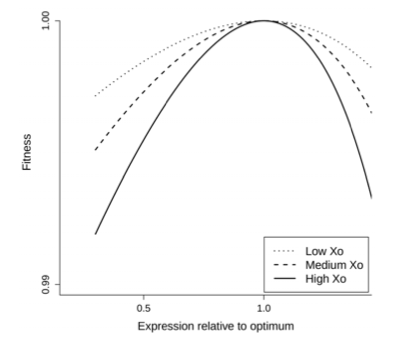
\includegraphics[width=2.5in]{FitnesVsexpression1.png} &
b)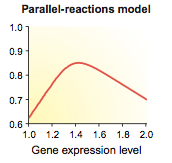
\includegraphics[width=2.5in]{FitnessVsExpression2.png}
\end{array}$
\end{center}
\caption{a): These curves represent the fitness function for different values of the optimal expression level $x_{0}$. They were generated assuming a benefit and cost functions, $B(x)$ and $C(x)$, where the x-axis is the expression level relative to the optimum. This graph was taken from \cite{Kahn2010}  b): Parallel reaction model in a gene metabolic network, where the vertical axis represents fitness. This graph was taken from\cite{Wang2011}.}
\label{Fig7.1}
\end{figure}

The non-monotonic form of fitness functions, leads to special properties when we examine the resulting distribution fitness from a protein distribution. To study these properties, we are going to use a simple triangular fitness function (Figure. \ref{Fig7.2}). With this testing function, we will measure the average fitness for several values of protein  variance.
\begin{figure}[H]
\begin{center}$
\begin{array}{cc}
a)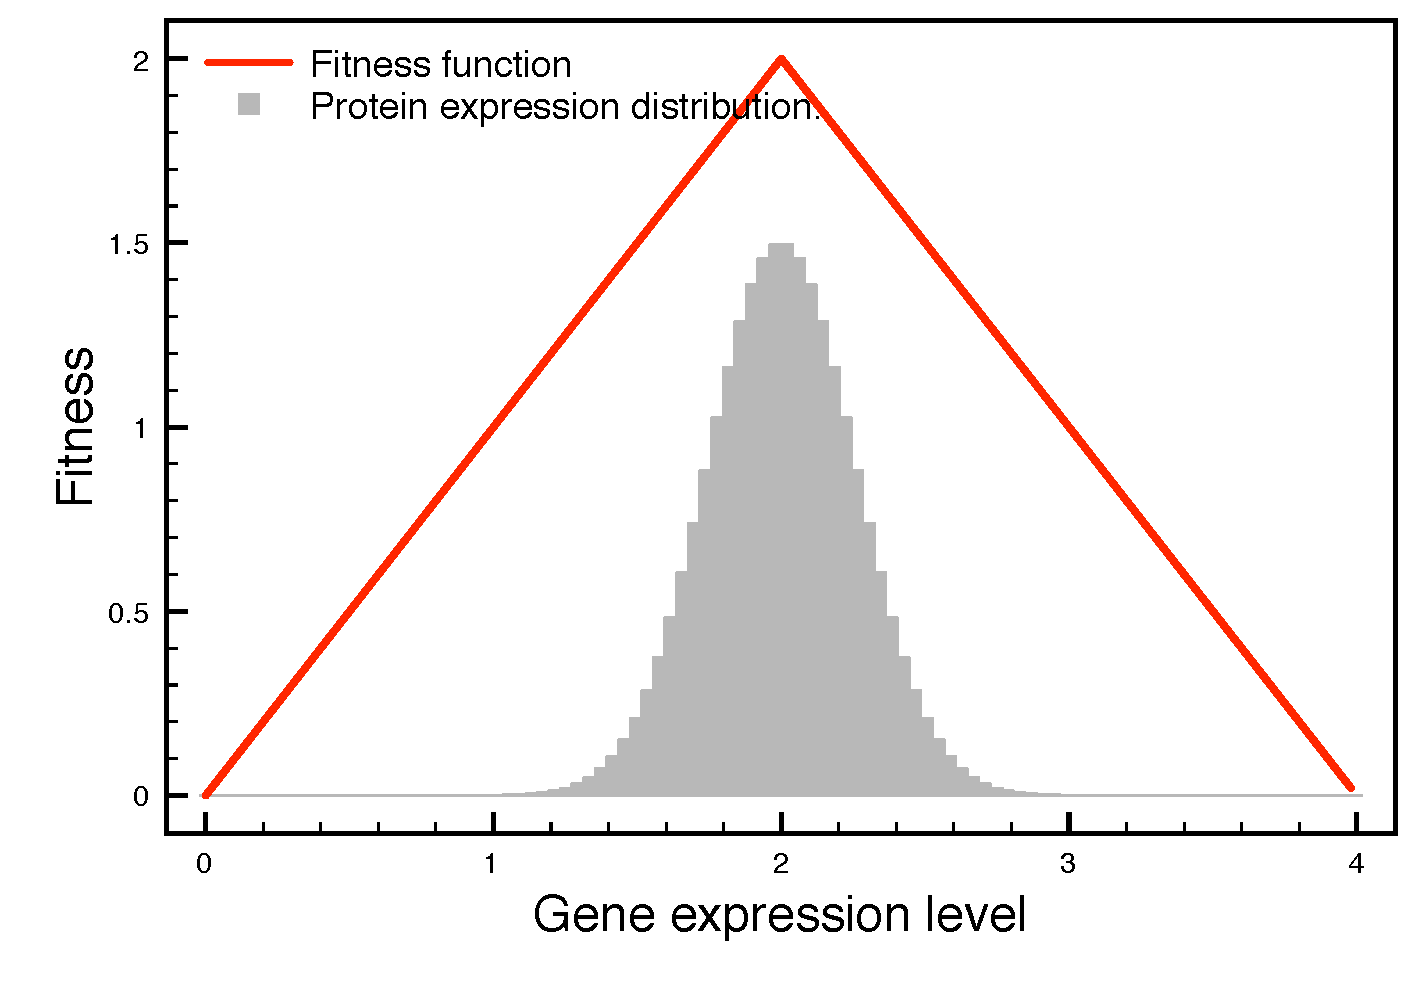
\includegraphics[width=2.5in]{triangularDistribution.pdf} &
b)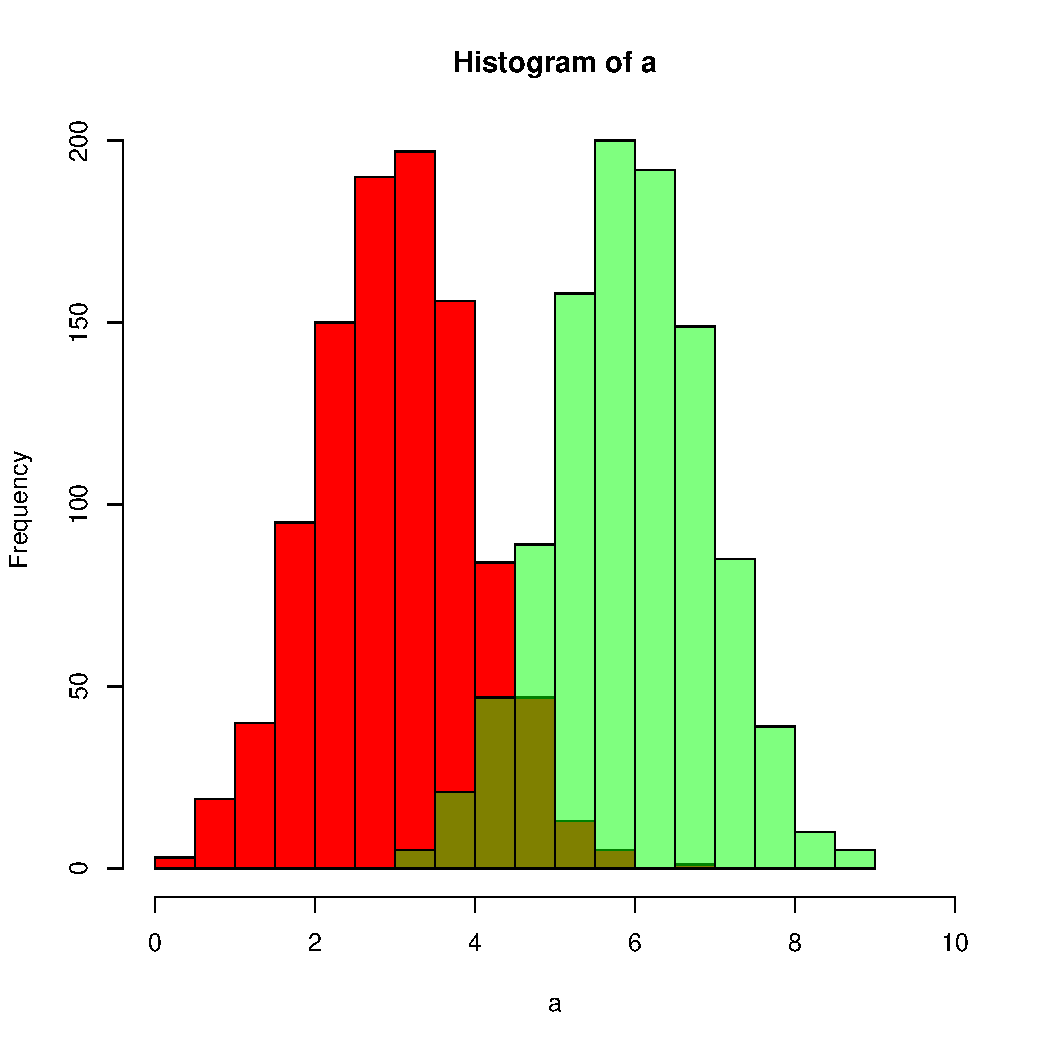
\includegraphics[width=2.5in]{Rplots.pdf}
\end{array}$
\end{center}
\caption{a): Triangular fitness function and an example of a distribution of protein expression with the form of a gaussian function. These functions are not taken from data of any biological system, they are a test tool to examine their effects on the stochastic simulation. b) In this figure is illustrated the fact that two different genes corresponding to two different phenotypes, have fitness distributions with different averages, where one phenotype is more advantageous than the other.}
\label{Fig7.2}
\end{figure}

In the next (Figure \ref{Fig7.3}) is shown the resulting fitness distribution for several  variance($\sigma$) values of the Gaussian protein distribution. 

\begin{figure}[H]
\begin{center}$
\begin{array}{cc}
a)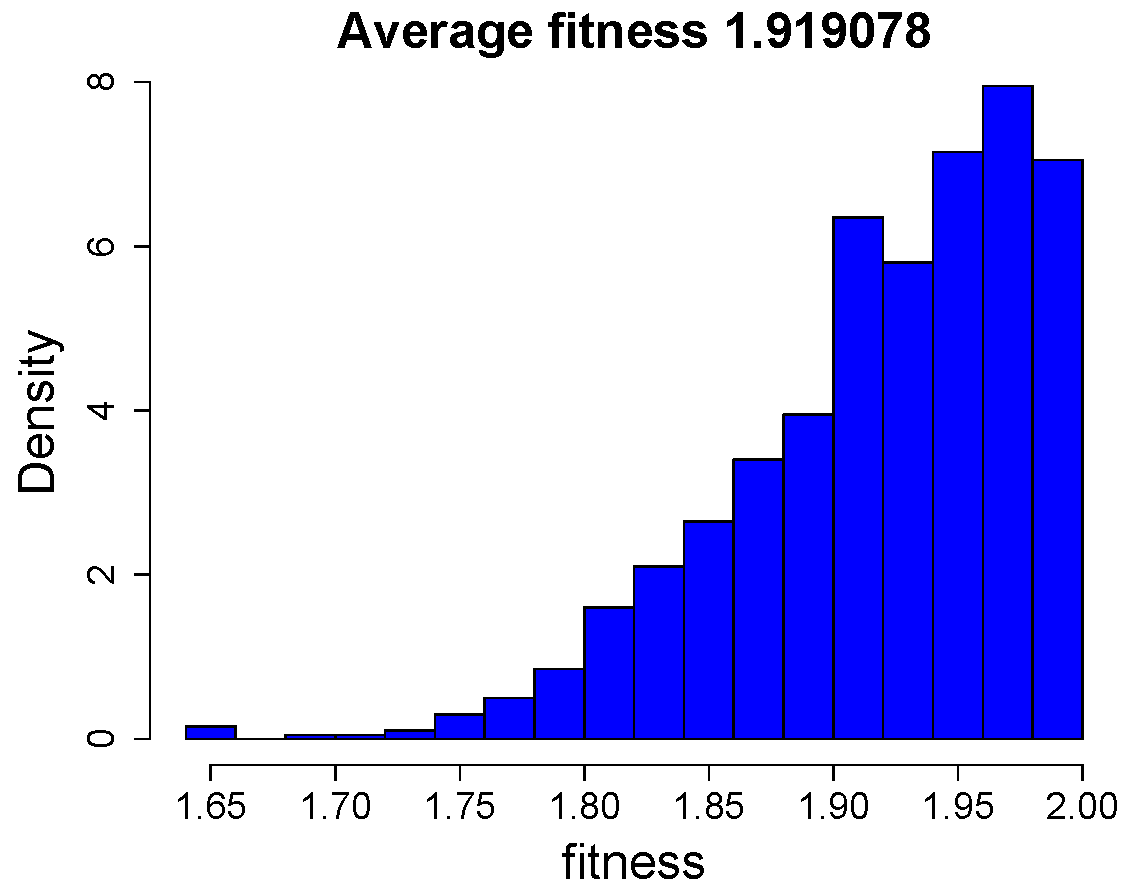
\includegraphics[width=2.5in]{triangularfitness01.pdf} &
b)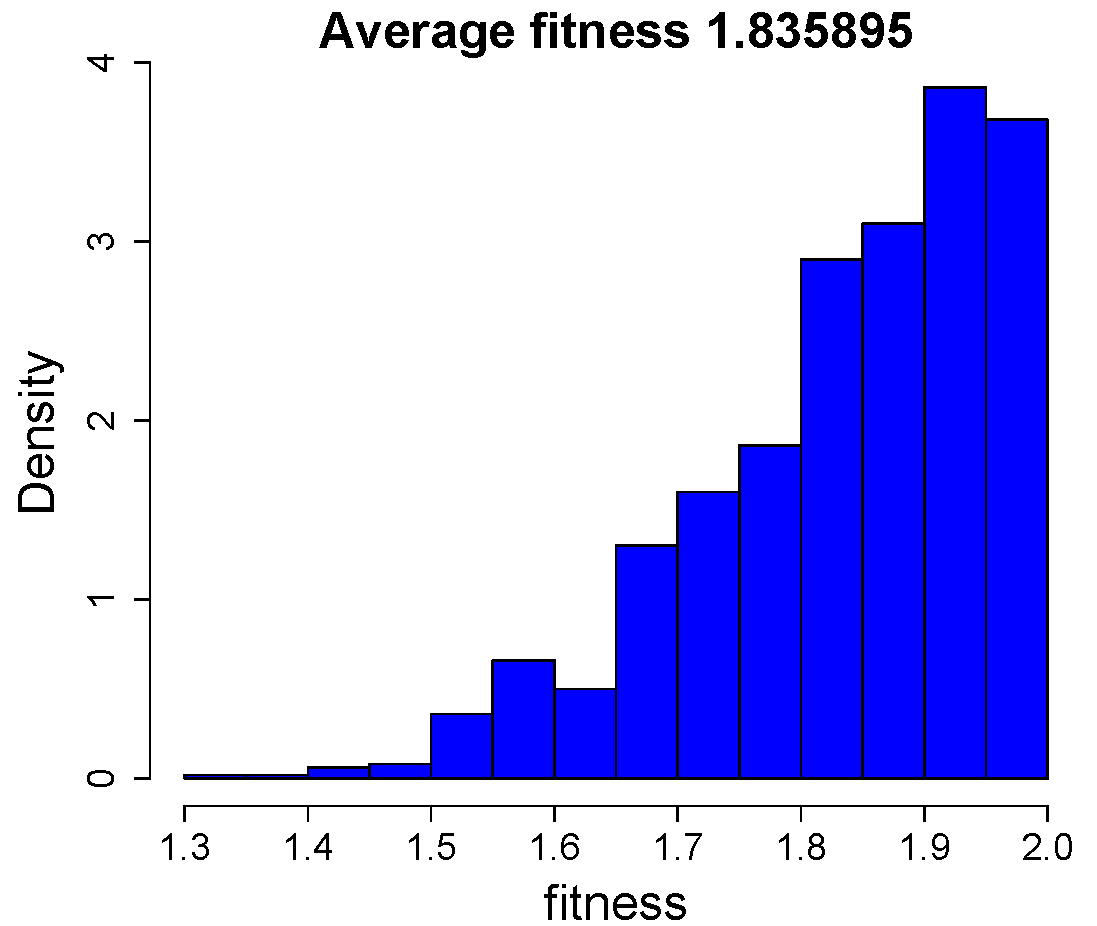
\includegraphics[width=2.5in]{triangularfitness02.pdf}\\
c)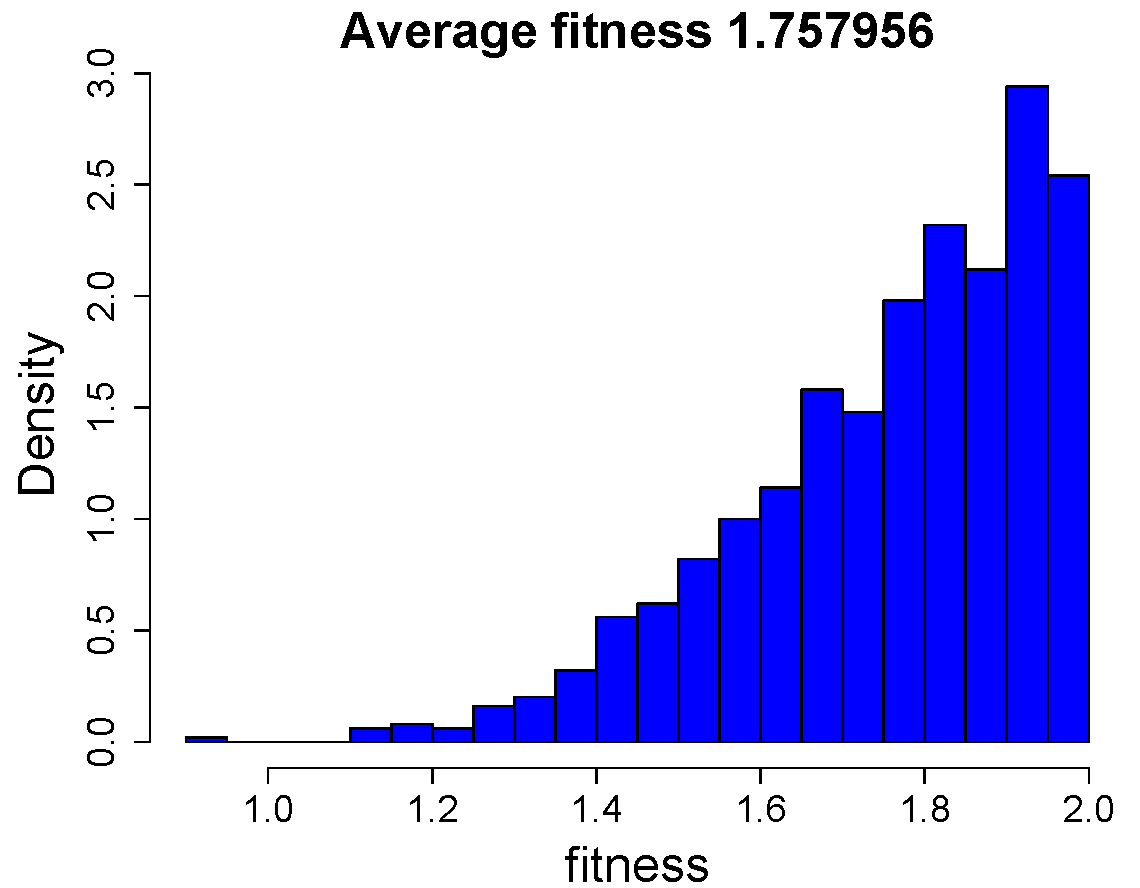
\includegraphics[width=2.5in]{triangularfitness03.pdf} &
d)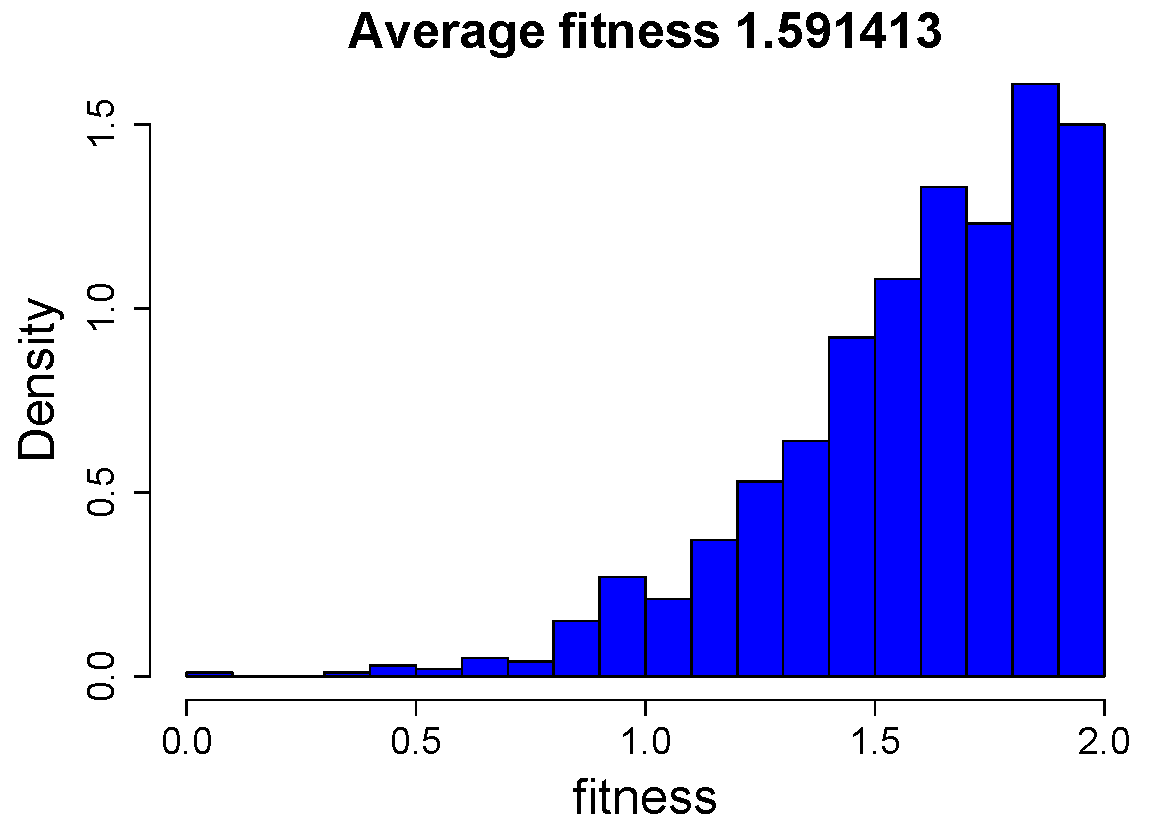
\includegraphics[width=2.5in]{triangularfitness05.pdf} 
\end{array}$
\end{center}
\caption{Fitness distributions resulting from the triangular function with optimum value $2$ and maximum fitness $2$ a) Protein expression variance $0.1$. b) Protein expression variance $0.2$. c) Protein expression variance $0.3$. d) Protein expression variance $0.5$.}
\label{Fig7.3}
\end{figure}

In (Figure \ref{Fig7.3}), is observed that average fitness decreases as variance increases. Now, the dependence of these two quantities will be examine in a graph of mean fitness versus variance $\sigma$ (Figure \ref{Fig7.4}). In this graph mean fitness has a lineal dependence with variance.
\begin{figure}[H]
  \begin{center}
    \leavevmode
    \ifpdf
      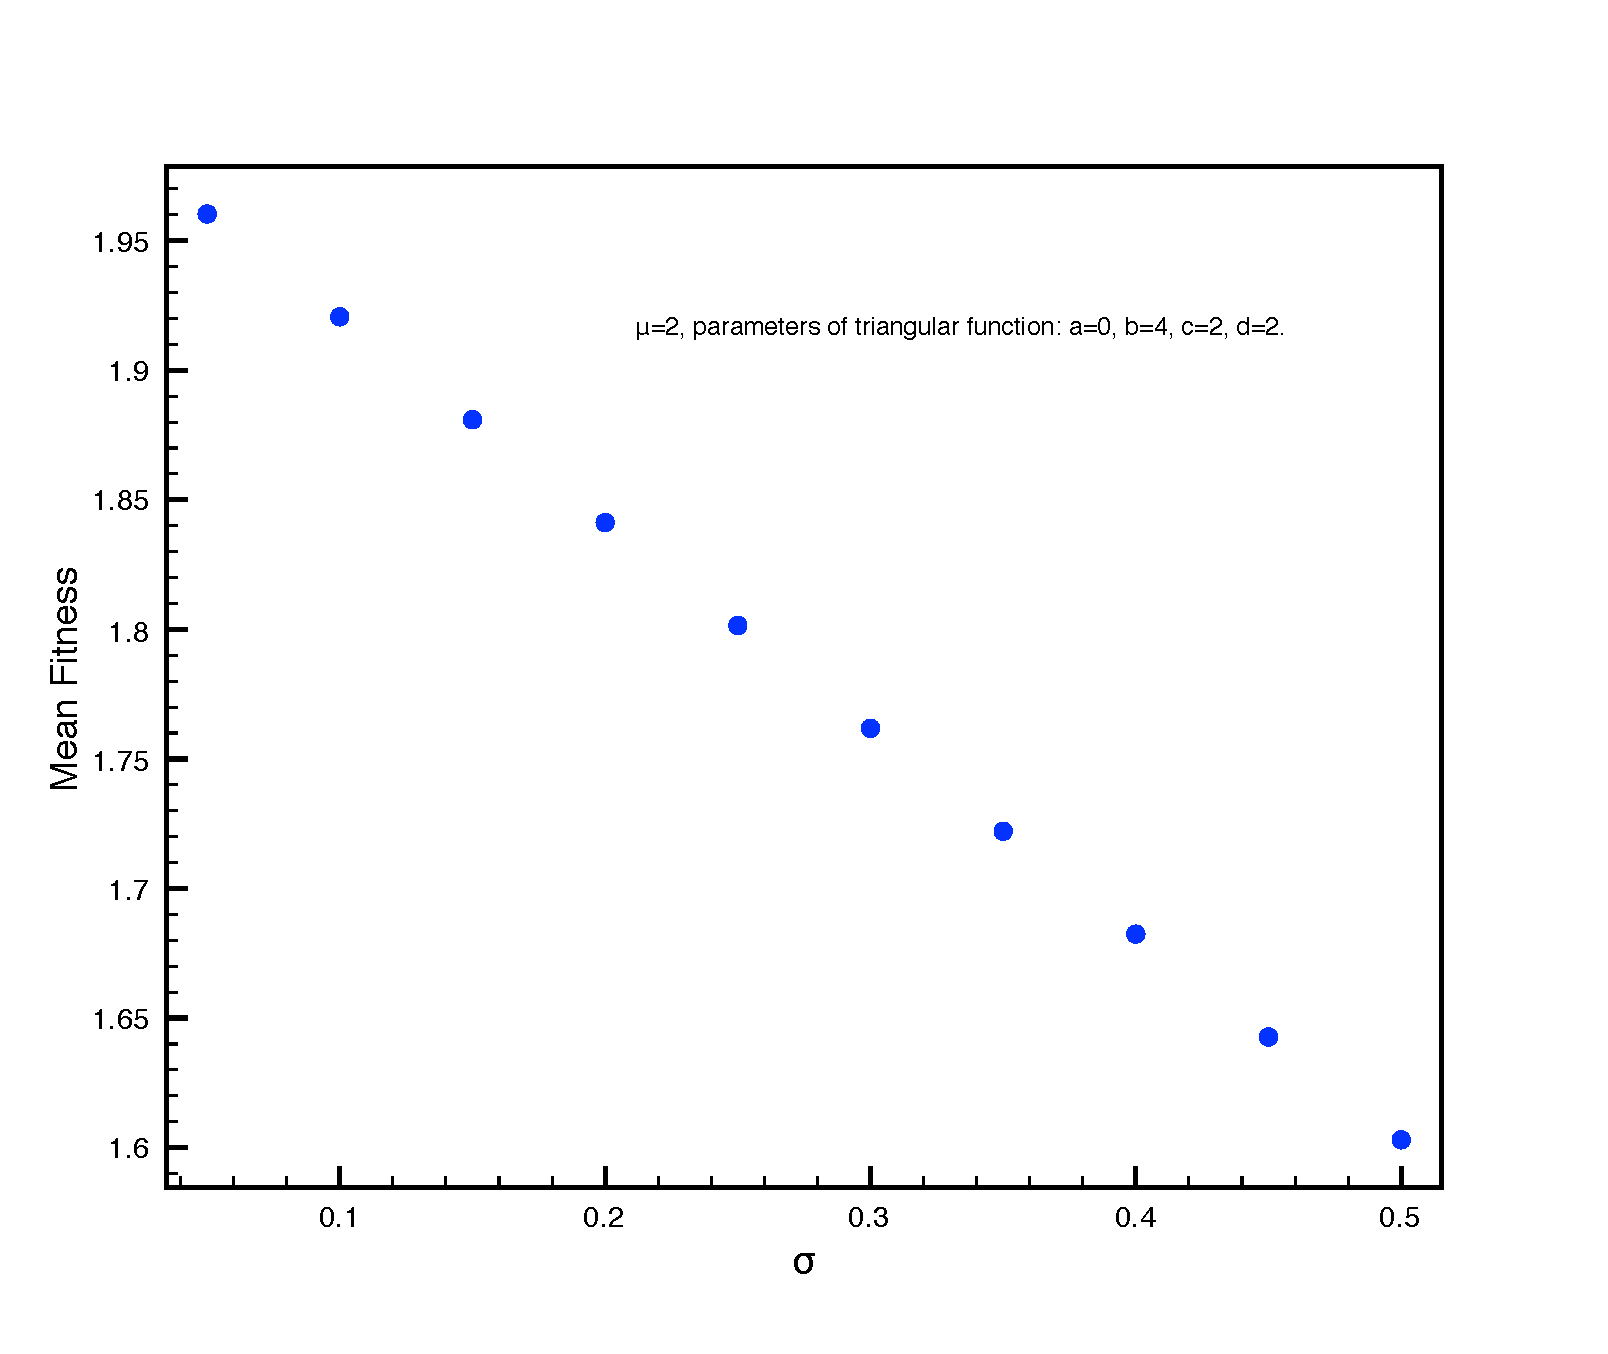
\includegraphics[width=9cm,height=8cm]{FitnessfunctionSigma.pdf}
    \else
      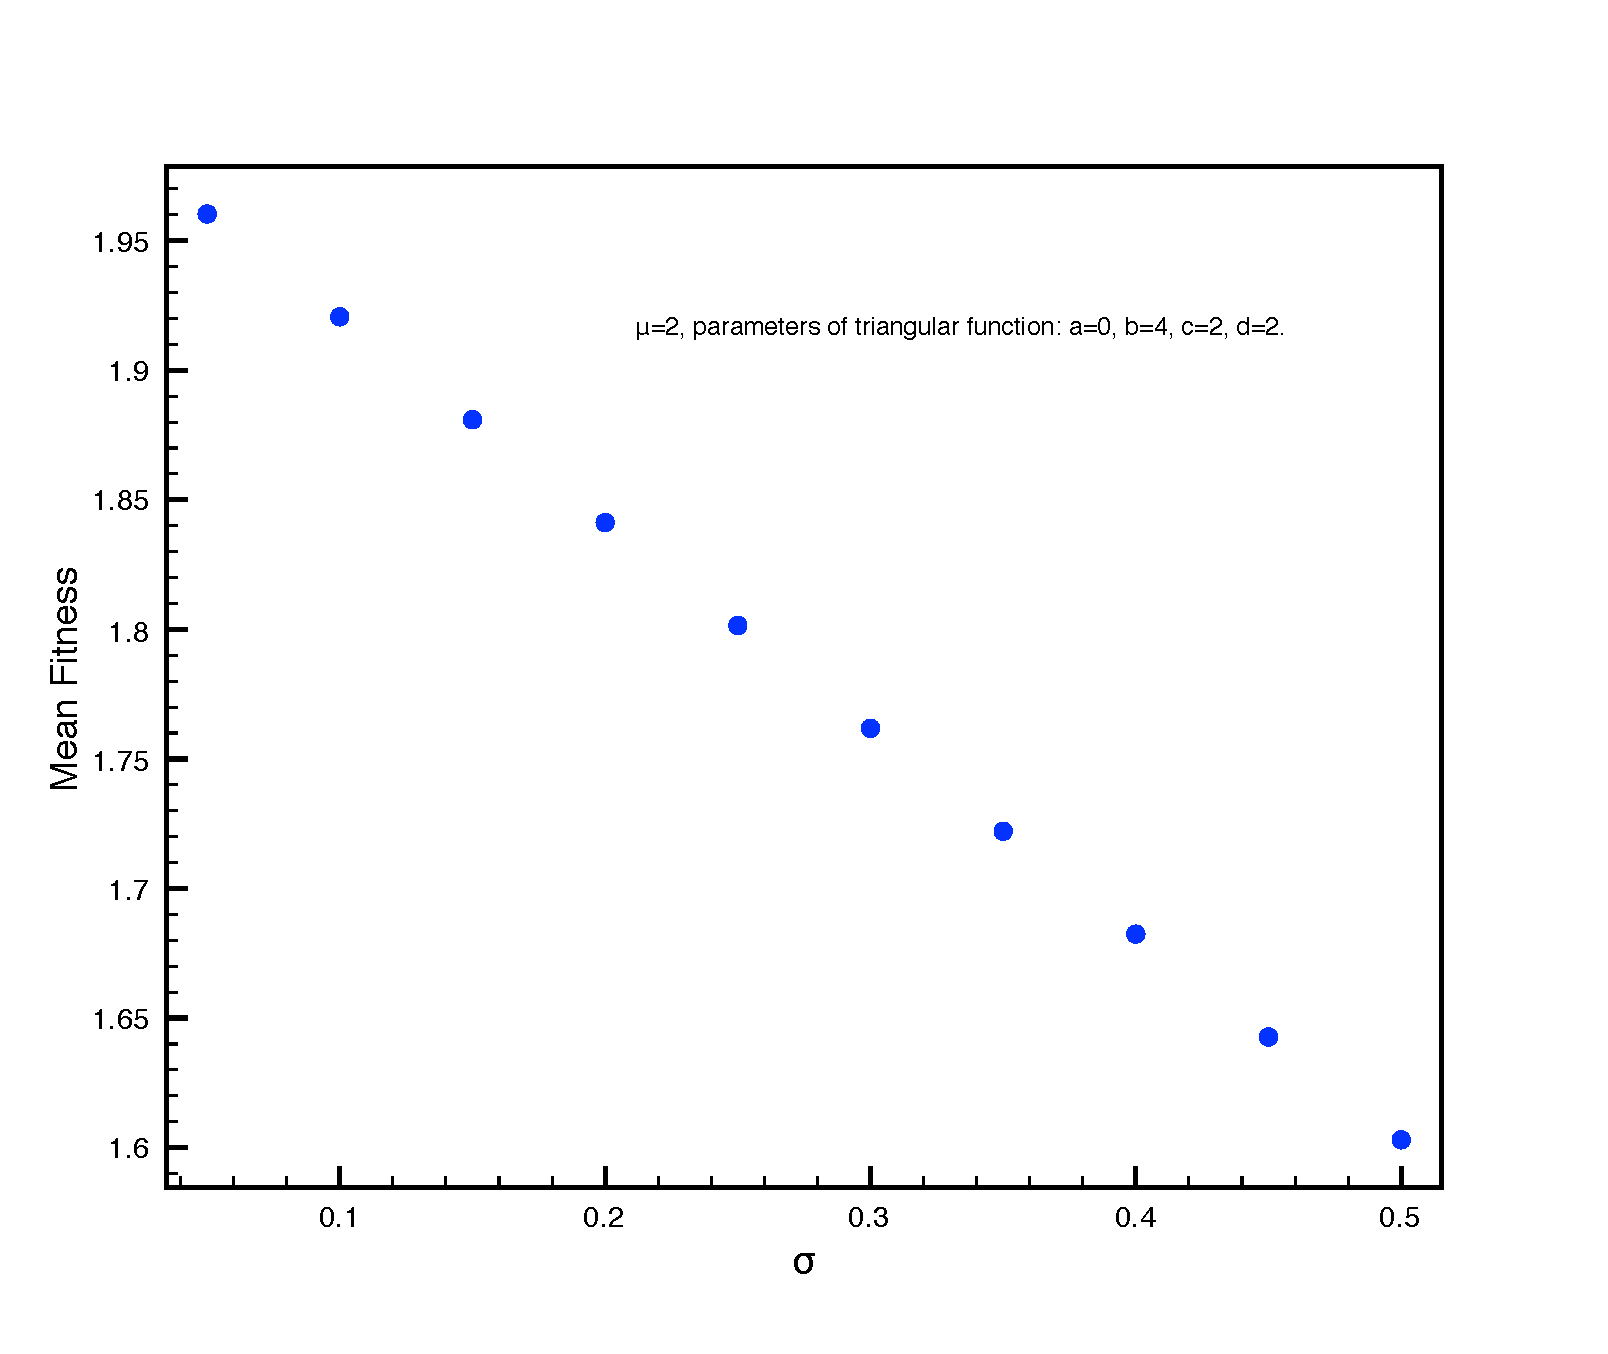
\includegraphics[width=9cm, height=8cm]{FitnessfunctionSigma.pdf}
    \fi
    \caption{Mean fitness dependence of protein variance.}
    \label{Fig7.4}
  \end{center}
  \end{figure}
The changes in  average fitness of the resulting distribution are a consequence of the non-monotonic form of fitness function. As a result, a symmetric  gaussian protein distribution generates an asymmetric fitness distribution with fitness decreasing as noise increases. Contrary, a linear increasing function have no effect on the symmetry and average of fitness as noise vary. These asymmetric resulting distributions can be classified in two types: humped toward left, and humped toward right (Figure. \ref{Fig7.4}).
\begin{figure}[H]
\begin{center}$
\begin{array}{cc}
a)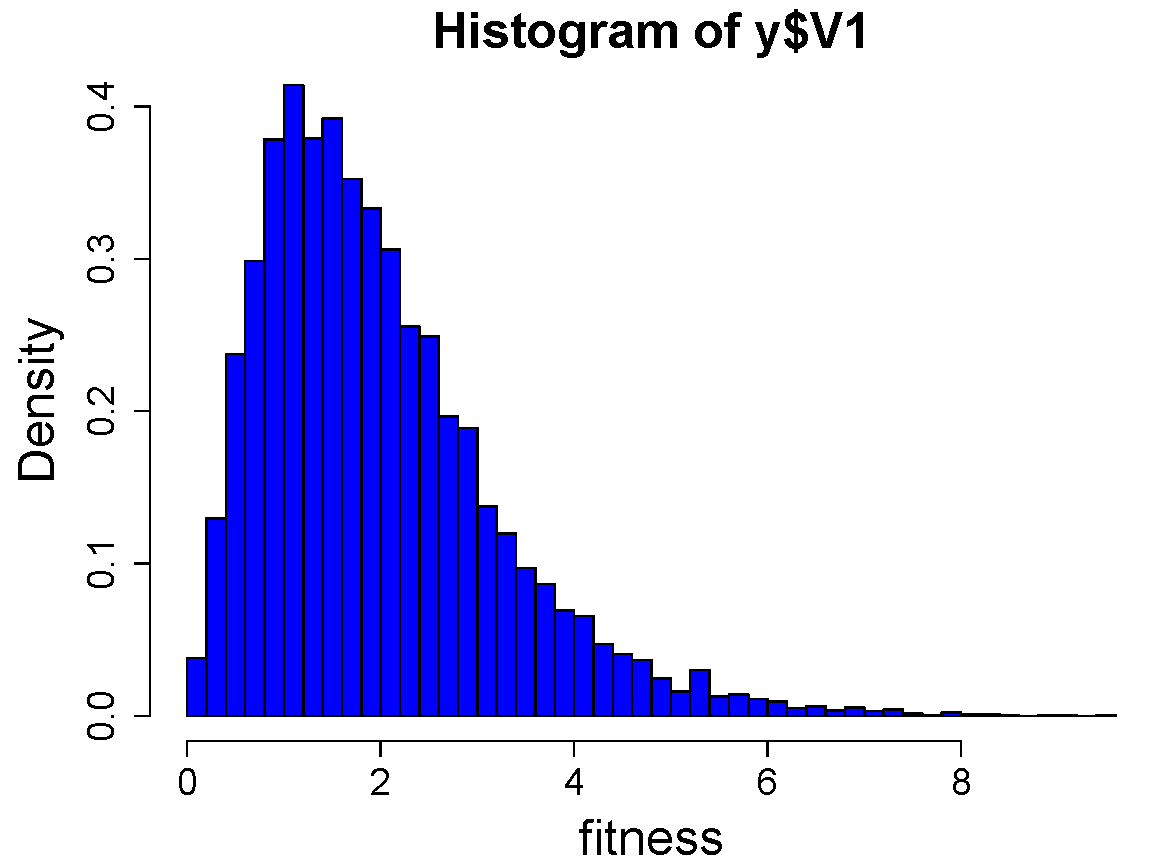
\includegraphics[width=2.5in]{humpedright.pdf} &
b)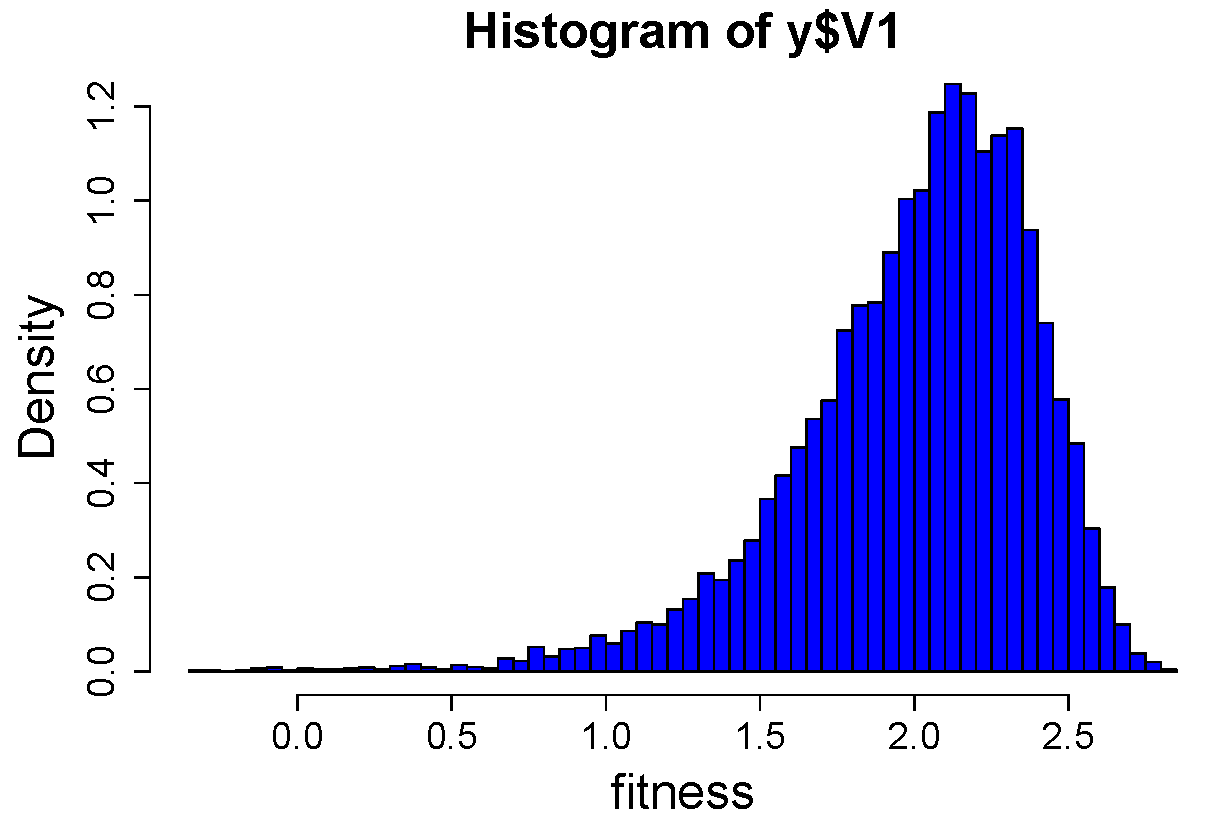
\includegraphics[width=2.5in]{humpedleft.pdf}
\end{array}$
\end{center}
\caption{a) Distribution humped toward left. These distributions characterizes because the mean is at the right hand of the mode(Gamma distribution with variance $0.3$). b) Distribution humped toward right(Extreme Value distribution with variance $0.3$). These distributions characterizes because the mean is at the left hand of the mode. The example distributions have mean equal $2$.}
\label{Fig7.4}
\end{figure}
The effects of the asymmetric shapes with growing  noise will be examine in the dynamics of moran process.

\section{Fixation Probability}
In this model model the fitness for the initial populations of individuals and their offsprings comes from a statistical distribution, which can be usually gaussian or poisson's, but for simplicity, we are initially  going to use a Gaussian distribution. Then, we will used asymmetric  distributions like gamma, to analyze the effects of symmetry in Moran process.

Let individuals of alleles of types $1$ and $0$ have values of fitness $f_{1i}$ and $f_{0j}$ respectively, that are random values from a fitness distribution. Then the probability that type $1$ is choosen for reproduction is
\begin{equation}
p_{reproduction}=\frac{\sum_{i=1}^{n}f_{1i}}{\sum_{i=1}^{n}f_{1i} + \sum_{j=1}^{N-n}f_{0j}}
\end{equation} 
where $n$ is the number of type $1$ individuals and $N$ the size of total population. Therefore the probabilities of transition are
\begin{equation}
P_{n,n+1}=\frac{\sum_{i=1}^{n}f_{1i}}{\sum_{i=1}^{n}f_{1i} + \sum_{j=1}^{N-n}f_{0j}}\frac{N-n}{N}
\end{equation}
\begin{equation}
P_{n,n-1}=\frac{\sum_{j=1}^{N-n}f_{0j}}{\sum_{i=1}^{n}f_{1i} + \sum_{j=1}^{N-n}f_{0j}}\frac{n}{N}
\end{equation}
replacing them in recursion equation
\begin{equation}
y_{n}=y_{n+1}\frac{P_{n,n+1}}{P_{n,n-1}},
\end{equation}
which leads to
\begin{equation}
y_{n}=y_{n+1}\frac{N-n}{n}\frac{\sum\limits_{i=1}^{n}f_{1i}}{ \sum\limits_{j=1}^{N-n}f_{0j}}.
\end{equation}
Since $y_1=\rho_1$, evaluating (31) for $n=1,2$ gives 
\begin{equation}
y_2 =\frac{\rho_1}{N-1}\frac{\sum\limits_{m=1}^{N-1}s_{m}}{\sum\limits_{m=1}^{1}r_{m}}
\end{equation}
\begin{equation}
y_3 =\frac{\rho_1}{N-1}\frac{\sum\limits_{m=1}^{N-1}s_{m}}{\sum\limits_{m=1}^{1}r_{m}}\frac{2}{N-2}\frac{\sum\limits_{m=1}^{N-2}s_{m}}{\sum\limits_{m=1}^{2}r_{m}}.
\end{equation}
Thus, by induction 
\begin{equation}
y_{i}=\rho_1\frac{(i-1)!(N-i)!}{(N-1)!}\prod\limits_{j=2}^{i}{\frac{\sum\limits_{m=1}^{N-(j-1)}s_m}{\sum\limits_{m=1}^{j-1}r_m}},\;\;\;\; i\geq 2.
\end{equation}
From the condition $\sum_{n=1}^{N}{y_n}=1-\rho_{1}$, the expression for $\rho_1$ is
\begin{equation}
1=\rho_1 + \sum\limits_{i=2}^{N}{\rho_1\frac{(i-1)!(N-i)!}{(N-1)!}\prod\limits_{j=2}^{i}{\frac{\sum\limits_{m=1}^{N-(j-1)}s_m}{\sum\limits_{m=1}^{j-1}r_m}}}
\end{equation}
\begin{equation}
\rho_1=\left(1 + \sum\limits_{i=2}^{N}{\frac{(i-1)!(N-i)!}{(N-1)!}\prod\limits_{j=2}^{i}{\frac{\sum\limits_{m=1}^{N-(j-1)}s_m}{\sum\limits_{m=1}^{j-1}r_m}}}\right)^{-1}
\end{equation}
For simplicity in the calculus of $\rho_{1}$ with this expression, we use $s_{m}$ as a deterministic variable. Therefore, the above equation reduces to

\begin{equation}
\rho_1=\left(1 + \sum\limits_{i=2}^{N}{(i-1)!s^{i-1}\prod\limits_{j=2}^{i}{\frac{1}{\sum\limits_{m=1}^{j-1}r_m}}}\right)^{-1}.
\end{equation}

Because $\rho_{1}$ is a function of the product among the sum of samples from a statistical distribution, $\rho_{1}$ is an stochastic variable, then we should calculated the average of $\rho_{1}$, which is the result that  simulation will give as fixation probability. The calculus of the average $\rho$ in terms of the mean and standard deviation  of the stochastic variable $r_{m}$ is really is a calculus of inferential statistics.
\section{Results}
\begin{figure}[H]
  \begin{center}
    \leavevmode
    \ifpdf
      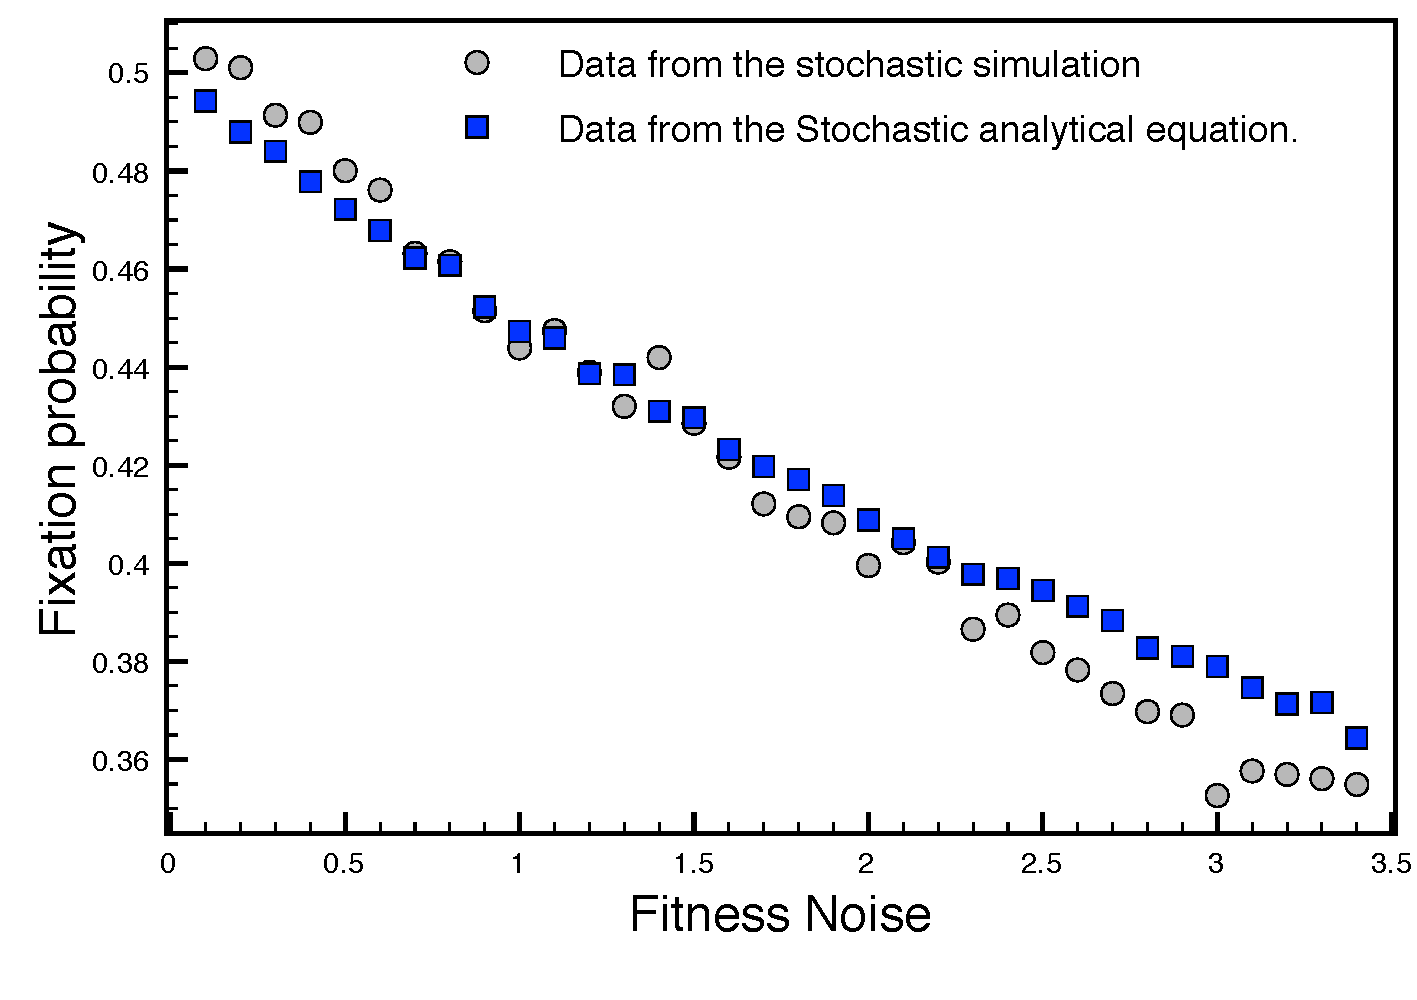
\includegraphics[width=9cm,height=8cm]{FixationProVsNoise.pdf}
    \else
      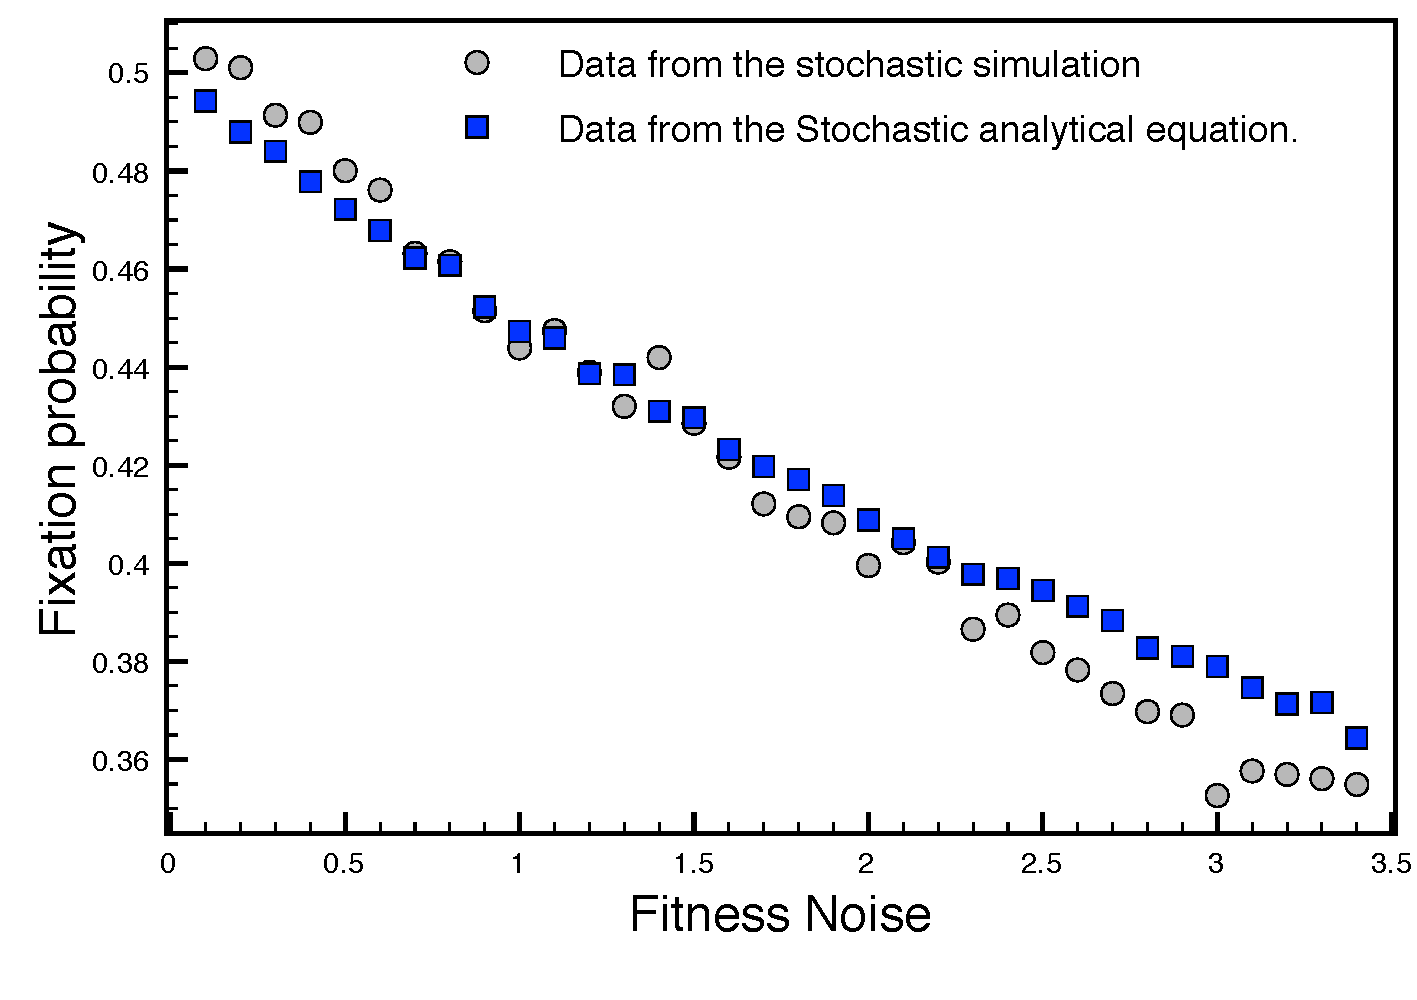
\includegraphics[width=9cm, height=8cm]{FixationProVsNoise.pdf}
    \fi
    \caption{Fixation probability for a mutant whose type has average fitness $\bar r=2$ as a function of fitness noise from a gamma distribution, in a population of size $n=100$ and individuals of fixed fitness $s=1$.}
    \label{}
  \end{center}
  \end{figure}
  
  
\begin{figure}[H]
  \begin{center}
    \leavevmode
    \ifpdf
      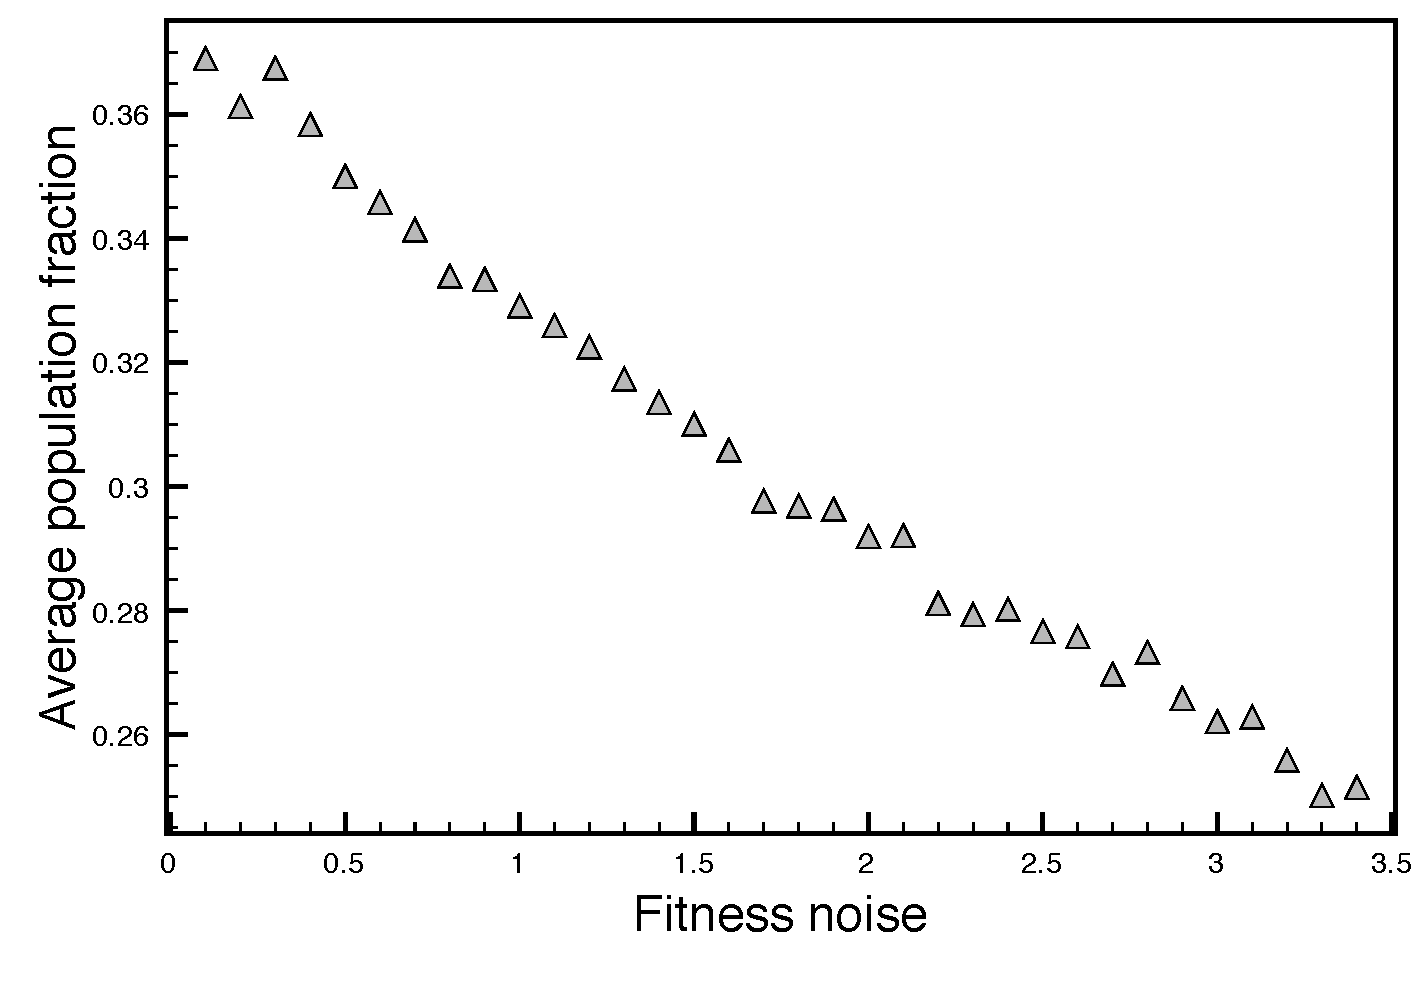
\includegraphics[width=9cm,height=8cm]{AveXti700Vsnoise.pdf}
    \else
      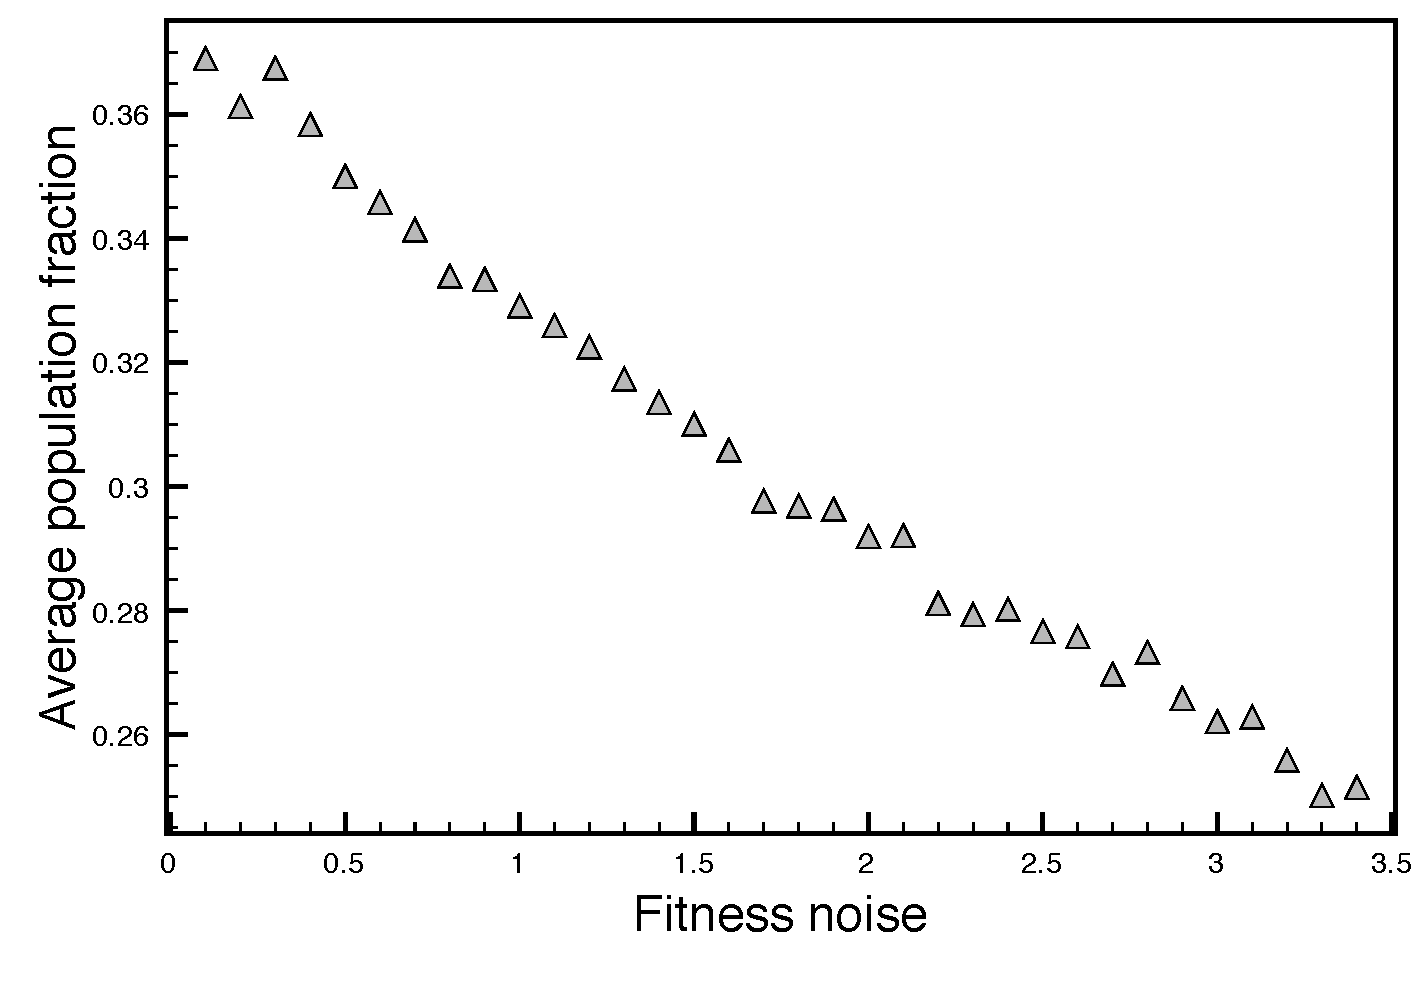
\includegraphics[width=9cm, height=8cm]{AveXti700Vsnoise.pdf}
    \fi
    \caption{$n=100$ $s=1$ $i=1$ gamma average $2$ Time $700$.}
    \label{}
  \end{center}
  \end{figure}
  
  \begin{figure}[H]
  \begin{center}
    \leavevmode
    \ifpdf
      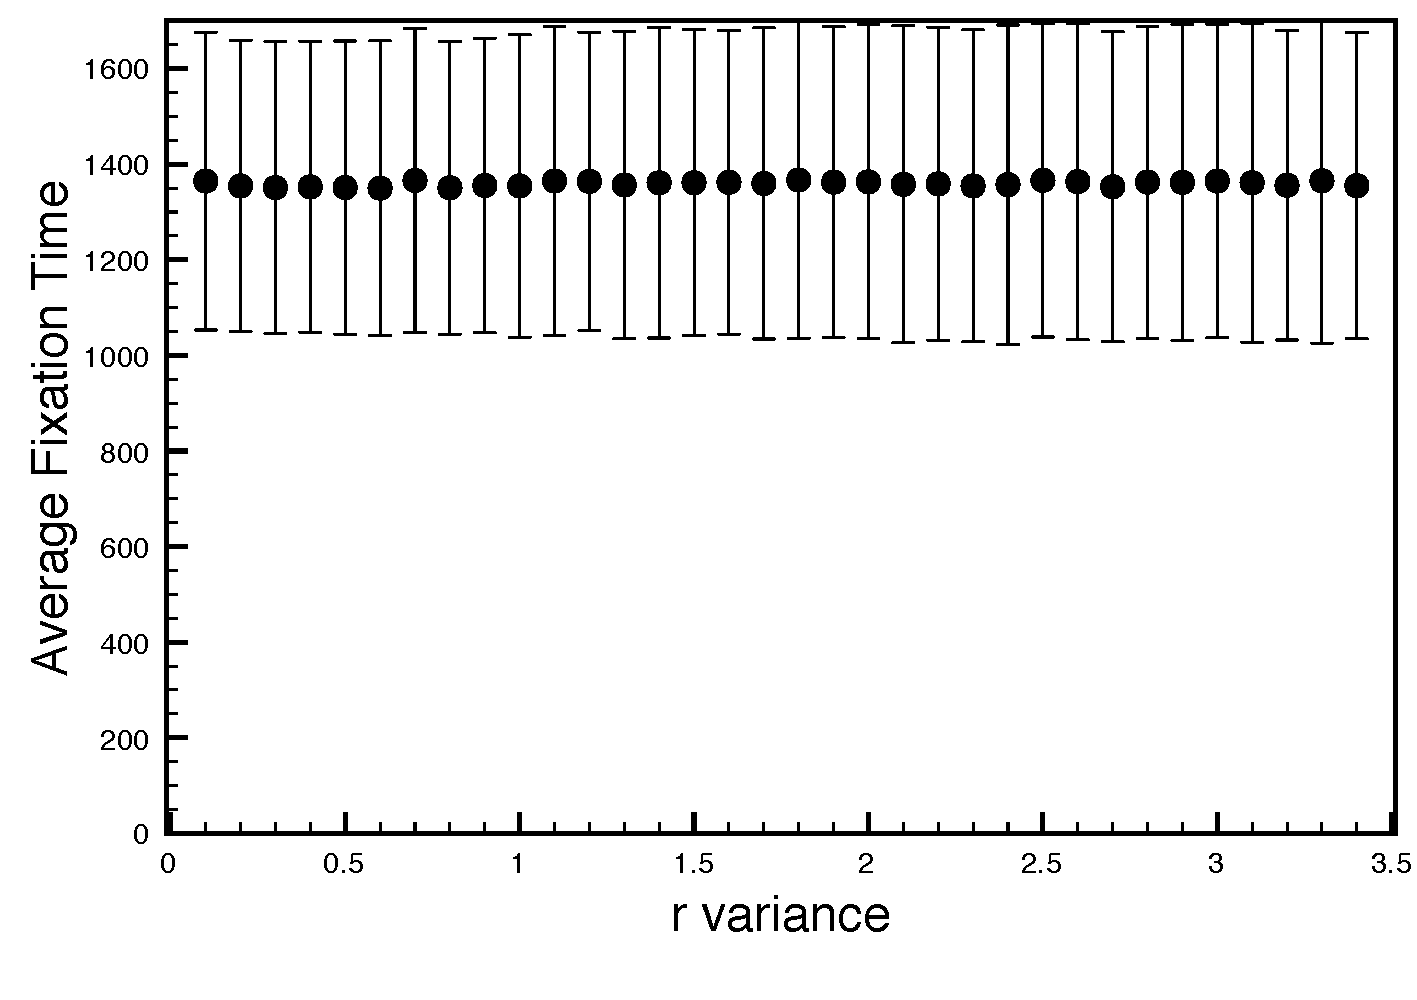
\includegraphics[width=9cm,height=8cm]{Averagefixationtimervariance1001.pdf}
    \else
      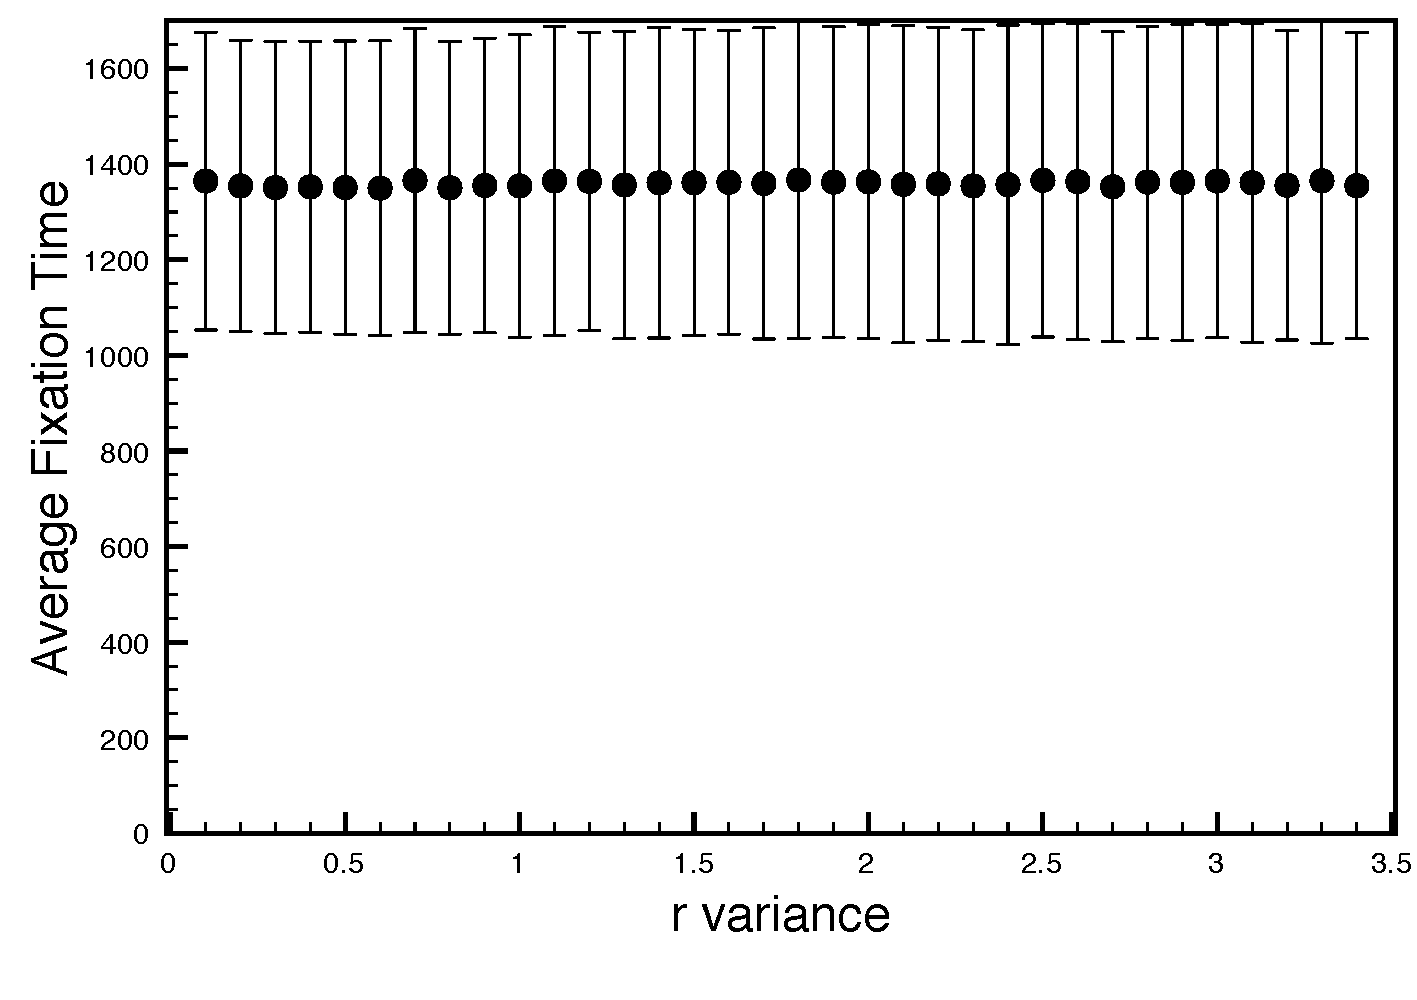
\includegraphics[width=9cm, height=8cm]{Averagefixationtimervariance1001.pdf}
    \fi
    \caption{$n=100$ $s=1$ $i=1$ gamma $r$ average $2$ .}
    \label{}
  \end{center}
  \end{figure}
  
  Fitness function of protein expression
\begin{figure}[H]
\begin{center}$
\begin{array}{cc}
a)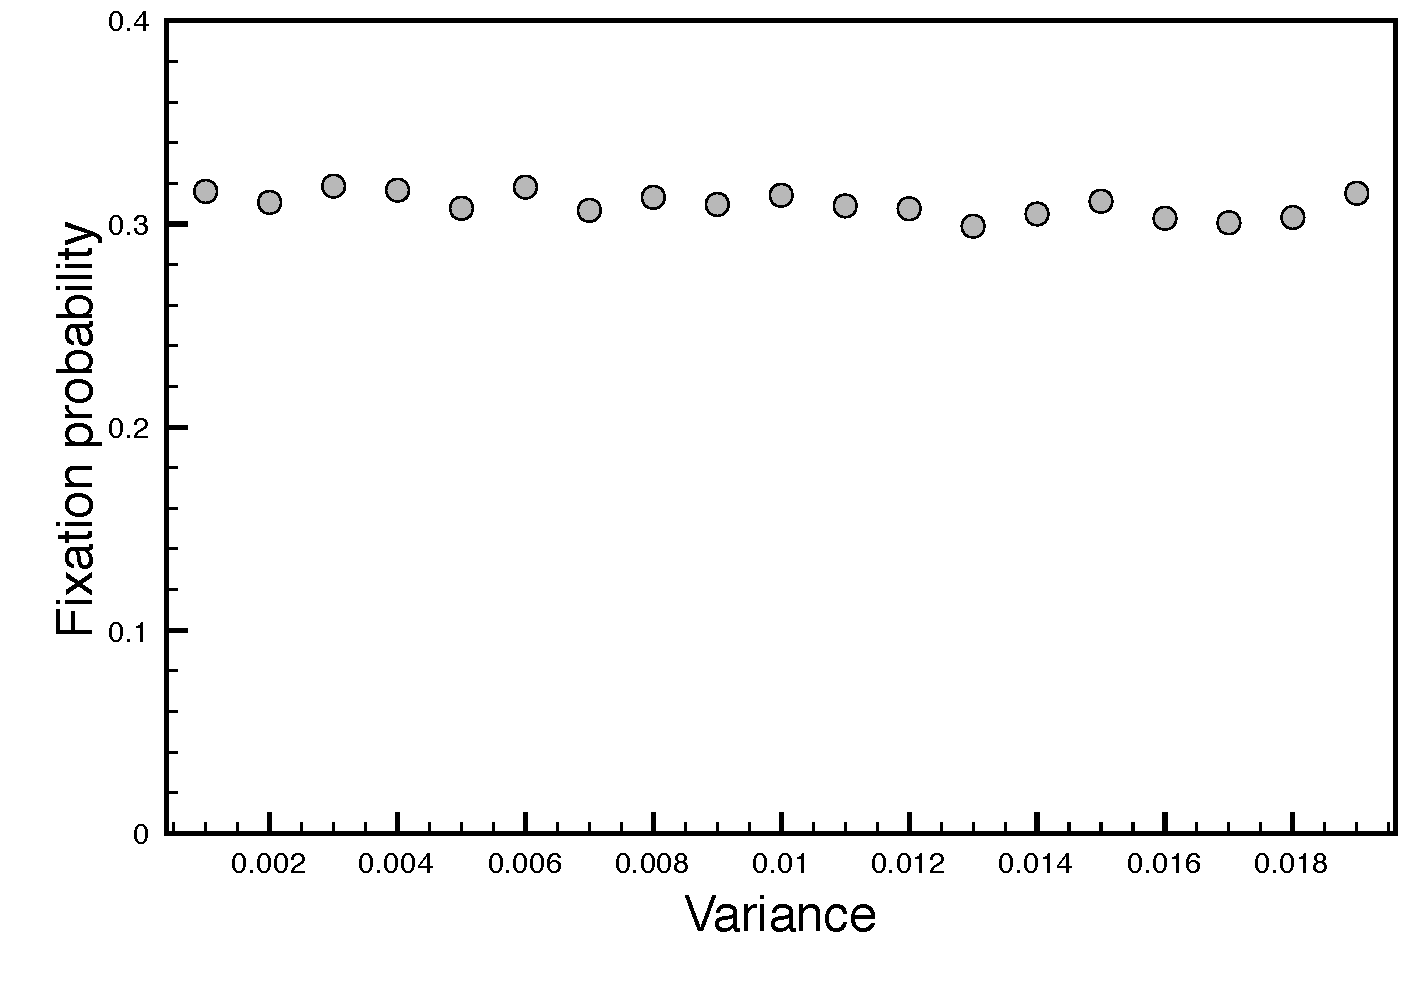
\includegraphics[width=2.5in]{exremeValueFixation.pdf} &
b)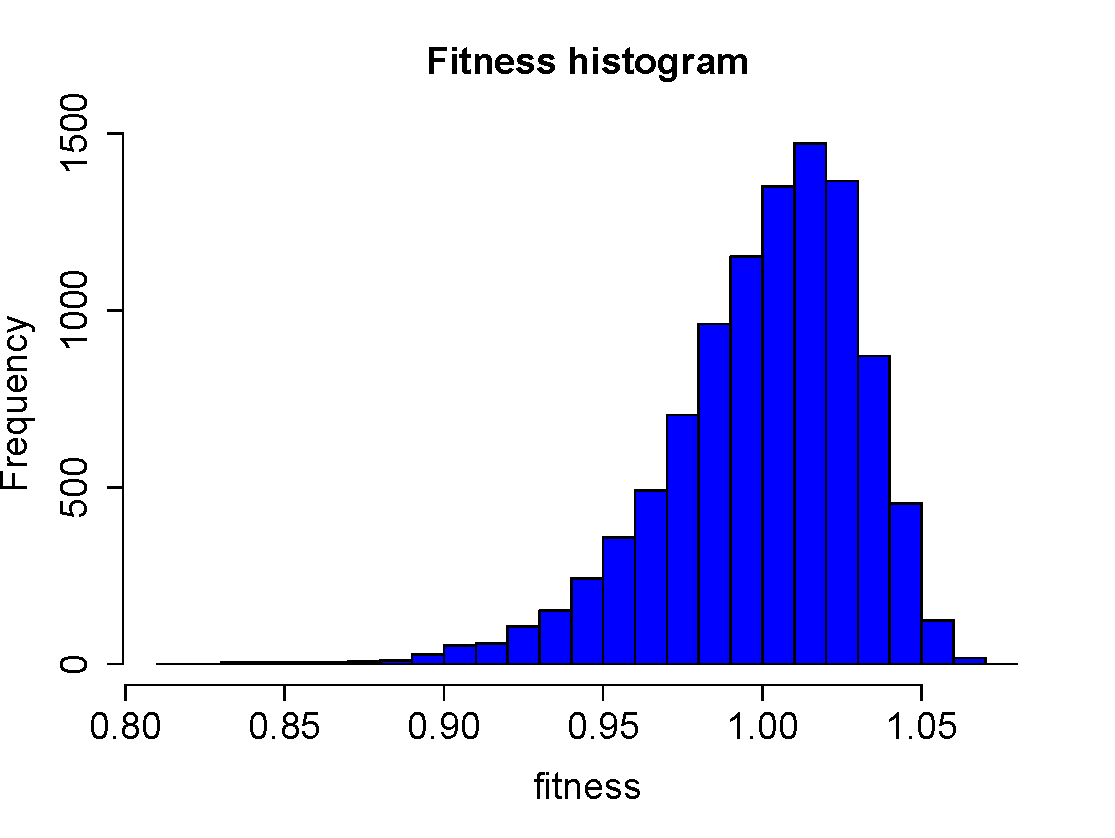
\includegraphics[width=2.5in]{histextremevalue.pdf}
\end{array}$
\end{center}
\caption{a): Fixation probability for increasing variance of a extreme value distribution, where $n=100$, $\bar{r}=1$, $s=0.7$ and initial population $i=1$. b) Extreme value distribution used in simulation for variance $0.001$. This distribution is humped toward right .}
\label{Fig7.2}
\end{figure}
Time fixation as a function of noise in protein level

  
\begin{figure}[H]
\begin{center}$
\begin{array}{cc}
a)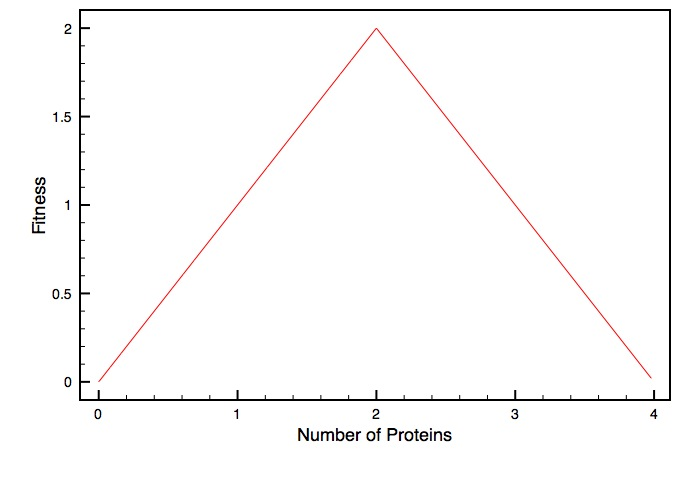
\includegraphics[width=2.5in]{TriangularFunction.jpg} &
b)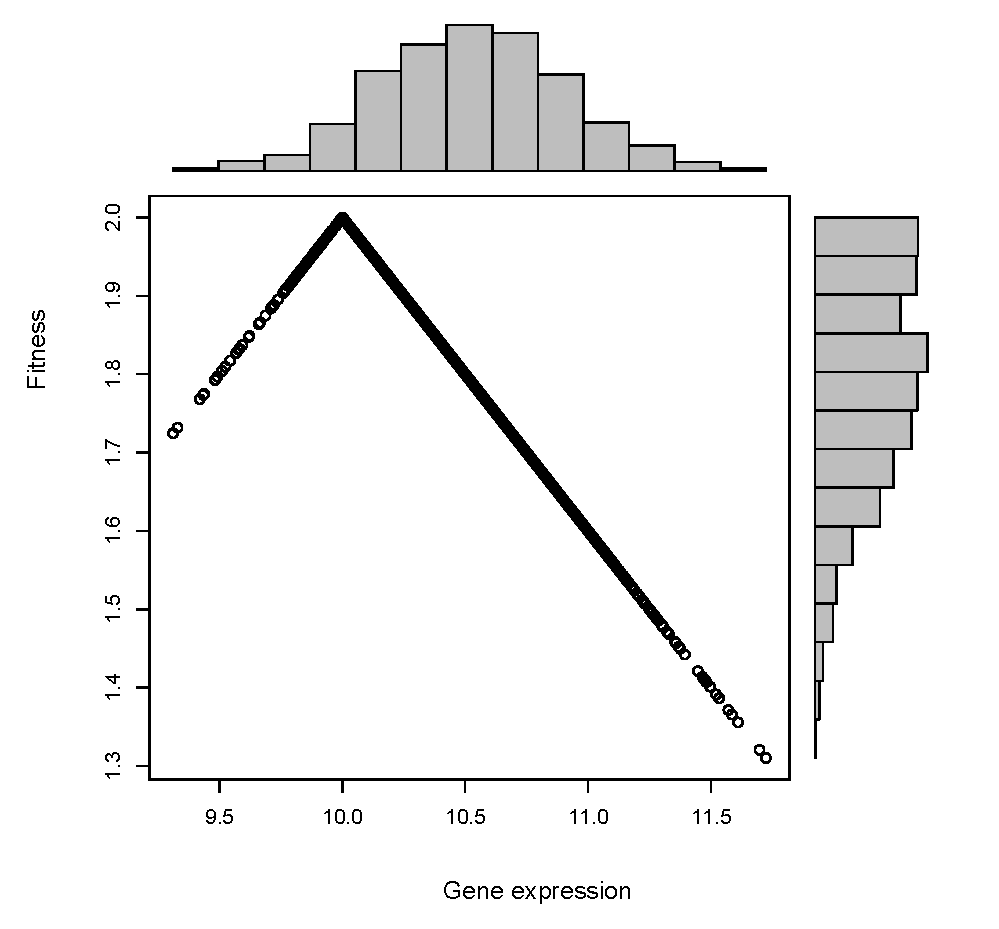
\includegraphics[width=2.5in]{triangularfunctionHistogram.pdf}
\end{array}$
\end{center}
\caption{a): Fitness triangular function of expression level. b): Resulting fitness distribution due to triangular function.}
\label{Fig7.2}
\end{figure}
Time fixation as a function of noise in protein level

  \begin{figure}[H]
\begin{center}$
\begin{array}{cc}
a) 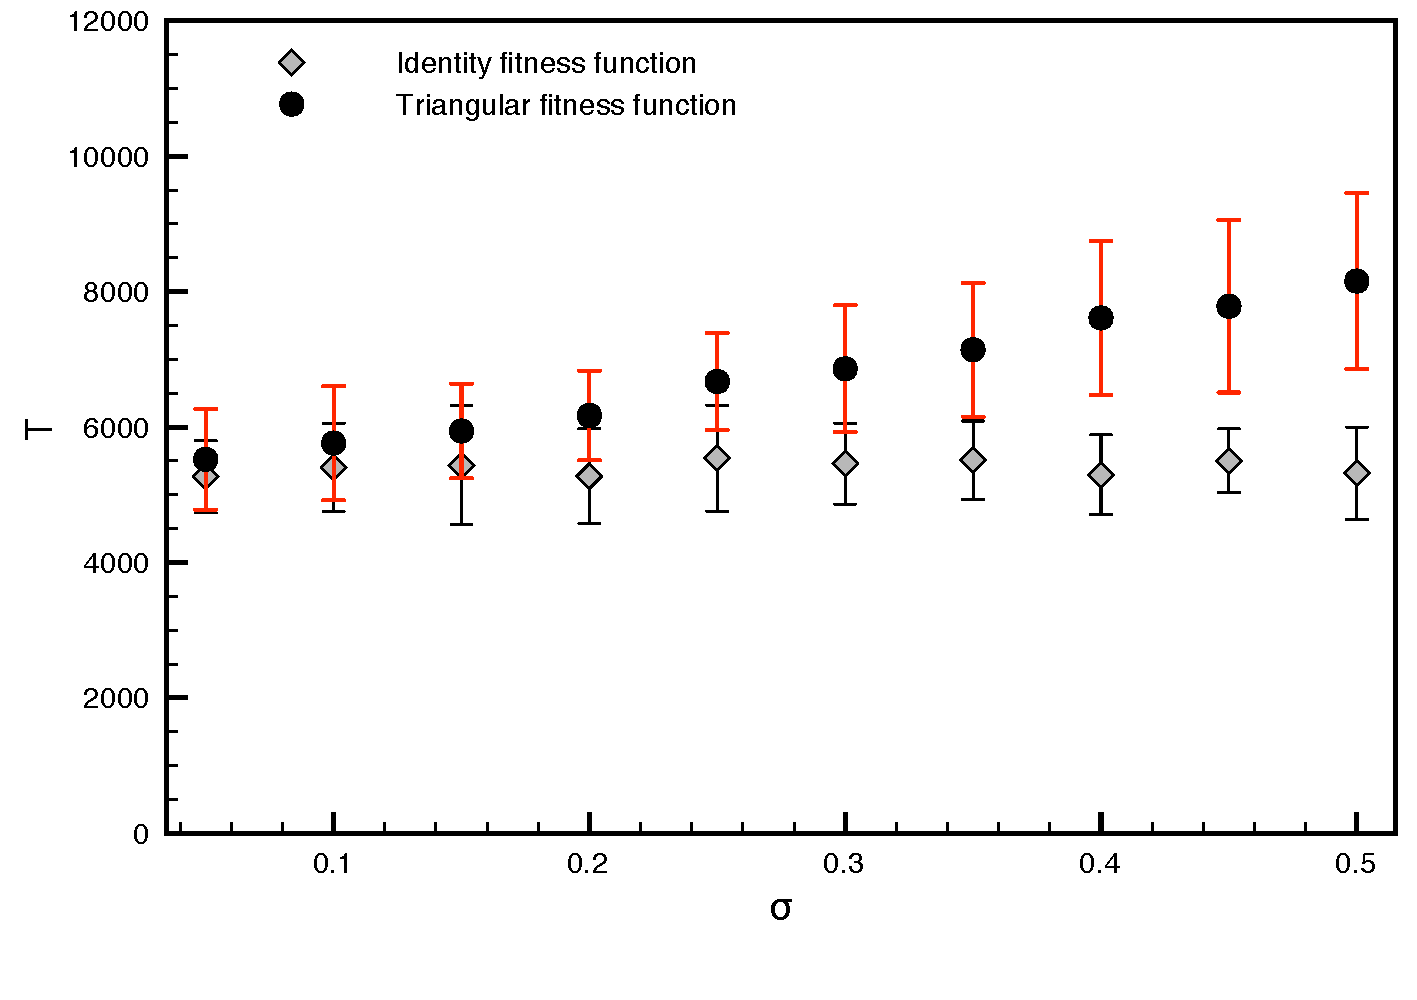
\includegraphics[width=2.5in]{SigmaVariationLTfitness.pdf} &
b)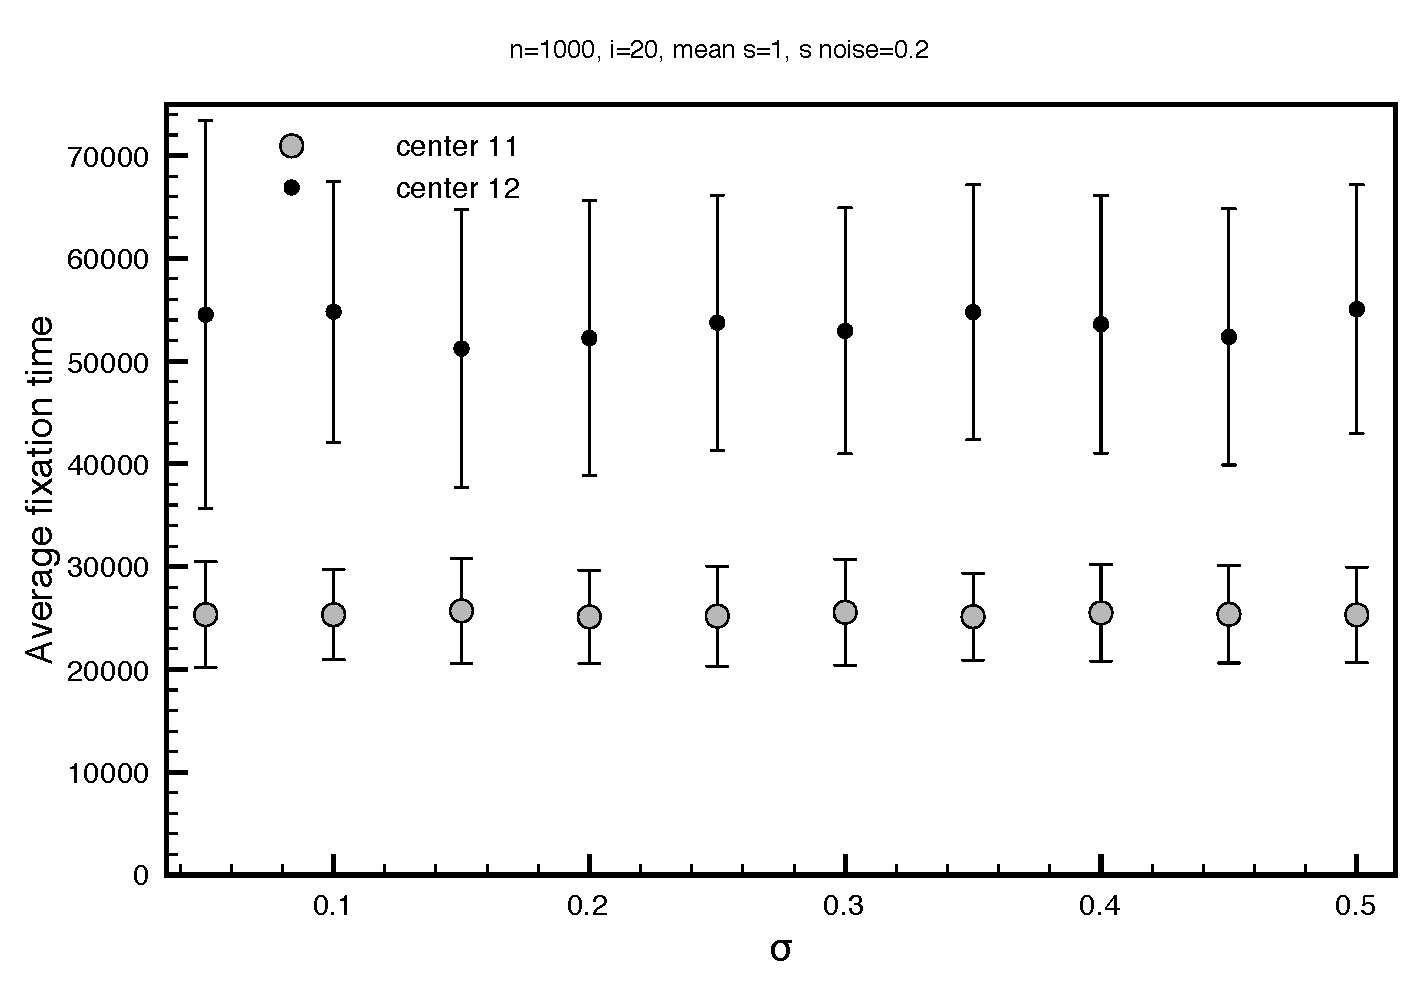
\includegraphics[width=2.5in]{nocenteredVsSigma.pdf}
\end{array}$
\end{center}
\caption{a): Average time when $10$ initial mutants(mean fitness=2) reach  $50\%$ of the population. This graph shows the average  time using a gaussian distribution with a linear function and with a non-linear function centered with the gaussian distribution. b): Average fixation time when the expression distribution is not centered with the fitness function. Fitness function centered on $10$ and distribution centered on $11$ and $12$.}
\label{Fig7.3}
\end{figure}
Really it is a function of average fitness of the distribution resulting from the fitness protein function.

\begin{figure}[H]
\begin{center}$
\begin{array}{cc}
a)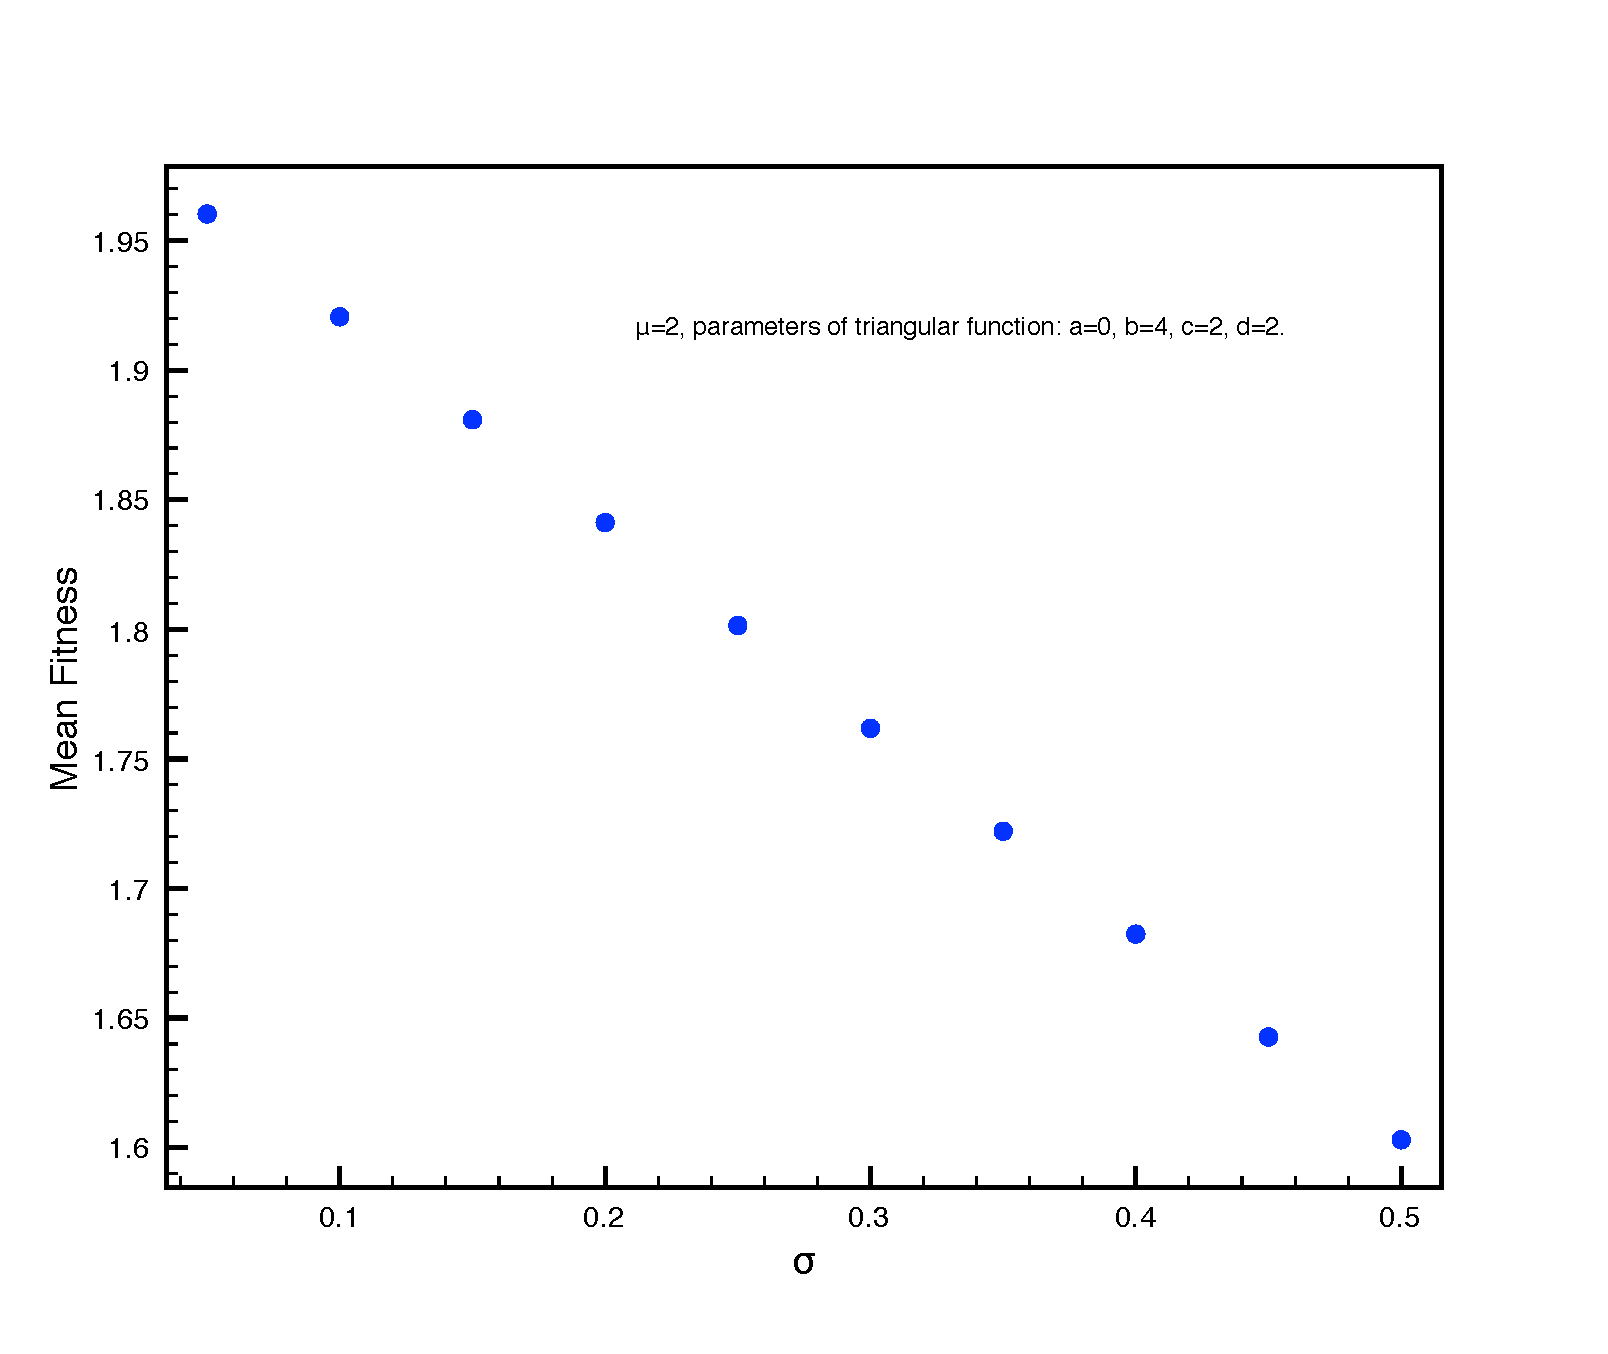
\includegraphics[width=2.5in]{FitnessfunctionSigma.pdf} &
b)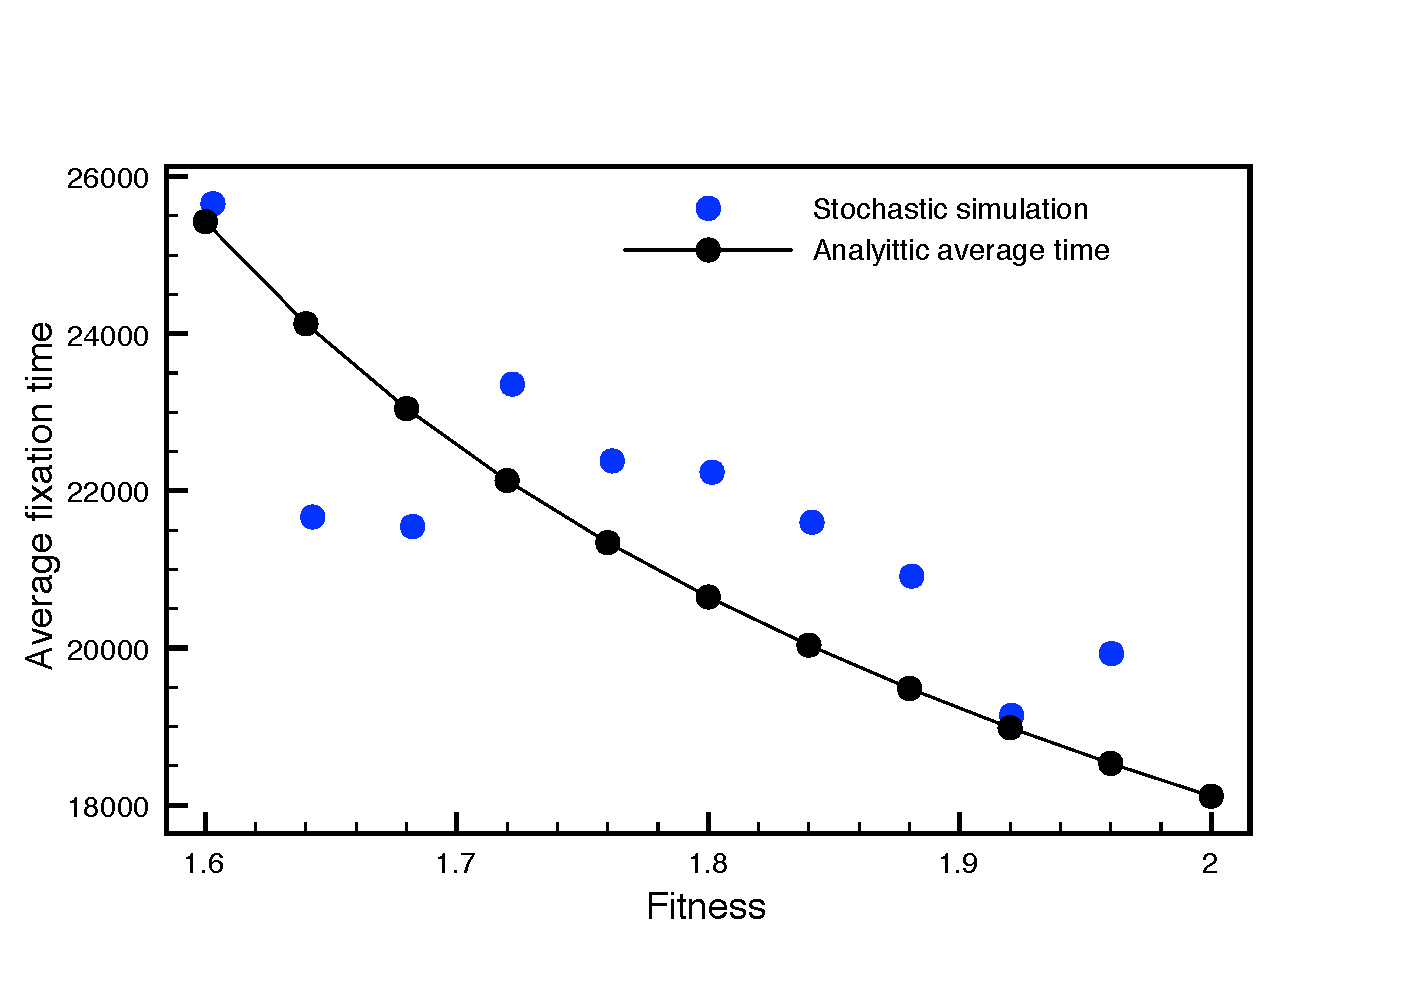
\includegraphics[width=2.7in]{AveragetimeFitness.pdf}
\end{array}$
\end{center}
\caption{a): Average resulting fitness from the triangular function as a function as the noise expression level. b): Average fixation time as a function of the mean fitness.}
\label{Fig7.4}
\end{figure}
See the average population fitness in time.
\section{The Fluctuation-Dissipation Theorem}
The fluctuation dissipation theorem is an approach to noise between different species in a stochastic system of coupled reactions. This theorem is based on the $\Omega$ expansion around to the stable points in  master equation\cite{Kampen}, which leads to a system of time differential equations for the variances of  different species in the stochastic system. The matrix formulation of this theorem is as follow\cite{Paulsson2005}  
\begin{equation}
\frac{d\boldsymbol{\sigma}}{dt}=\mathbf{A}\boldsymbol{\sigma} + \boldsymbol{\sigma}\mathbf{A}^{T} + \mathbf{B}
\end{equation}
where $\sigma_{ij}$ are the covariances and
\begin{equation}
A_{ij}=\frac{\partial}{\partial \langle n_j \rangle}\frac{\partial\langle n_i\rangle}{\partial t}\;\; ,\;\; B_{ij}=\sum\limits_{k}v_{jk}v_{ik}R_{k}
\end{equation}
$n_{i}$ are the quantities involved in the stochastic process. $B_{ii}$ is the sum of fluxes for each species $n_{i}$. When there are no equation for terms of the form$\partial_t\langle n_i n_j\rangle$, which represent events that change two different species simultaneously, $B_{ij}=0$\cite{Paulsson2005}. 

As an example to learn how  this theorem works, we can solve these equations in a system of protein synthesis from mRNA, where the average number of proteins is denoted by $\langle x\rangle$ and the mRNA by $\langle y\rangle$. They follow the dynamics.
\begin{equation}
\partial_{t}\langle y\rangle=\lambda_{1}- \beta_{1}\langle y\rangle
\end{equation}  
\begin{equation}
\partial_{t}\langle x \rangle=\lambda_{2}\langle y\rangle - \beta_{2}\langle x\rangle
\end{equation}
thus
\begin{equation}
\mathbf{A}=
\begin{pmatrix}
-\beta_1 & 0 \\
\lambda_2 & -\beta_2
\end{pmatrix}\;\; , \;\; \mathbf{B}=\begin{pmatrix} \lambda_1 + \beta_1 \langle y\rangle & 0 \\
0 & \lambda_2\langle y\rangle+ \beta_2\langle x\rangle\end{pmatrix}
\end{equation}
Finally the matrix for time derivates of variances is
\begin{equation}
\begin{pmatrix} \partial_{t} \sigma_{y}^{2} & \partial_t \sigma_{xy}\\
\partial_t \sigma_{xy} & \partial_t \sigma_{x}^{2}
\end{pmatrix}
=
\begin{pmatrix} -2\sigma_{yy}\beta_{1}+\beta_1\langle y\rangle+\lambda_1 & \lambda_2\sigma_{yy}-\sigma_{yx}\beta_2-\beta_1\sigma_{xy}\\
\lambda_2\sigma_{yy}-\sigma_{yx}\beta_2-\beta_1\sigma_{xy} & \lambda_2\langle y\rangle-\beta_2 \langle x\rangle + 2(\lambda_2\sigma_{xy}-\beta_2\sigma_{xx})
\end{pmatrix}
\end{equation}
Thus the respective differential equations for each variance are

\begin{gather}
\frac{d \sigma_{y}^{2}}{dt}=-2\sigma_{yy}\beta_1 + \beta_1 \langle y\rangle + \lambda_1\;\;, \;\; \frac{d\sigma_{xy}}{dt}= \lambda_2\sigma_{yy}-\sigma_{yx}\beta_2-\beta_1\sigma_{xy} \notag \\
\frac{d\sigma_{x}^{2}}{dt}=\lambda_2\langle y\rangle-\beta_2 \langle x\rangle + 2(\lambda_2\sigma_{xy}-\beta_2\sigma_{xx})
\end{gather}
In steady state the noise $\eta_{x}^{2}=\sigma_{x}^{2}/\langle x\rangle^2$ for proteins is related with mRNA noise $\eta_{y}^{2}=1/\langle y\rangle$ by the equation
\begin{equation}
\eta_{x}^{2}=\frac{1}{\langle x\rangle} +\frac{1}{\langle y\rangle(1+\beta_1/\beta_2)}.
\end{equation} 
In this equation we can see the intrinsic poissonian noise $1/\langle x\rangle$ and the external noise; the second term, which is the mRNA poissonian noise scaled by factor that depends on the degradation rates. This noise relation can also be  derived using the moment generating function\cite{Pedraza1}.
\section{Fluctuation-Dissipation Theorem for Random Drift and Stochastic Fitness}
In random drift two types of organisms with fitnesses $r$ and $s$ compete in population of fixed size $n$. In this system, the population fraction $\langle x\rangle$ of individuals with fitness $r$  follow sthe time differential equation
\begin{equation}
\frac{d \langle x\rangle}{dt}=\frac{r\langle x\rangle(1-\langle x\rangle)}{n(r\langle x\rangle + s(1-\langle x\rangle))}-\frac{s\langle x\rangle(1-\langle x\rangle)}{n(r\langle x\rangle + s(1-\langle x\rangle))},
\end{equation} 
where for simplicity we are going to use $\langle x\rangle=\bar{x}$.

The first two derivatives respect to $\bar{x}$ for the probability fluxes of this equation are:
\begin{equation}
\frac{\partial}{\partial\bar{x}}\frac{d\bar{x}}{dt}=\frac{r-s}{n}\left[\frac{(1-2\bar{x})(r\bar{x}+s(1-\bar{x}))-\bar{x}(1-\bar{x})(r-s)}{\left(r\bar{x}+s(1-\bar{x})\right)^{2}}\right]
\end{equation} 
\begin{equation}
\frac{\partial^{2}}{\partial\bar{x}^{2}}\frac{d\bar{x}}{dt}=\left[\frac{(2\bar{x}(s-r)-2s)(r\bar{x}+s(1-\bar{x}))-2(r-s)(s-\bar{x}^{2}(r-s)-2\bar{x}s)}{\left(r\bar{x}+s(1-\bar{x})\right)^{3}}\right]
\end{equation}
Thus the differential equation for $\sigma_{xx}$ in the case of fixed fitness is
\begin{equation}\label{7.22}
\frac{d\sigma_{xx}}{dt}=2\sigma_{xx}\frac{r-s}{n^2}\left[\frac{(1-2\bar{x})(r\bar{x}+s(1-\bar{x}))-\bar{x}(1-\bar{x})(r-s)}{\left(r\bar{x}+s(1-\bar{x})\right)^{2}}\right] + \frac{\bar{x}}{n^{2}}\frac{(1-\bar{x})(r+s)}{r\bar{x}+s(1-\bar{x})},
\end{equation}
where the general equation for $\sigma_{ij}$ has been divided by $n$ because generally in literature the time step $dt$ is rescale to $dt/n$. This was done to have compatibility with simulations, where time is not rescale to  size $n$ of the system. In the next (Figure \ref{Fig7.5}), the solution of Eq. \eqref{7.22} is plotted with different simulations for random drift with deterministic fitness and noise fitness. It is observed that the variance differential equations has  maximum value at similar times in the simulation.  
\begin{figure}[H]
  \begin{center}
    \leavevmode
    \ifpdf
      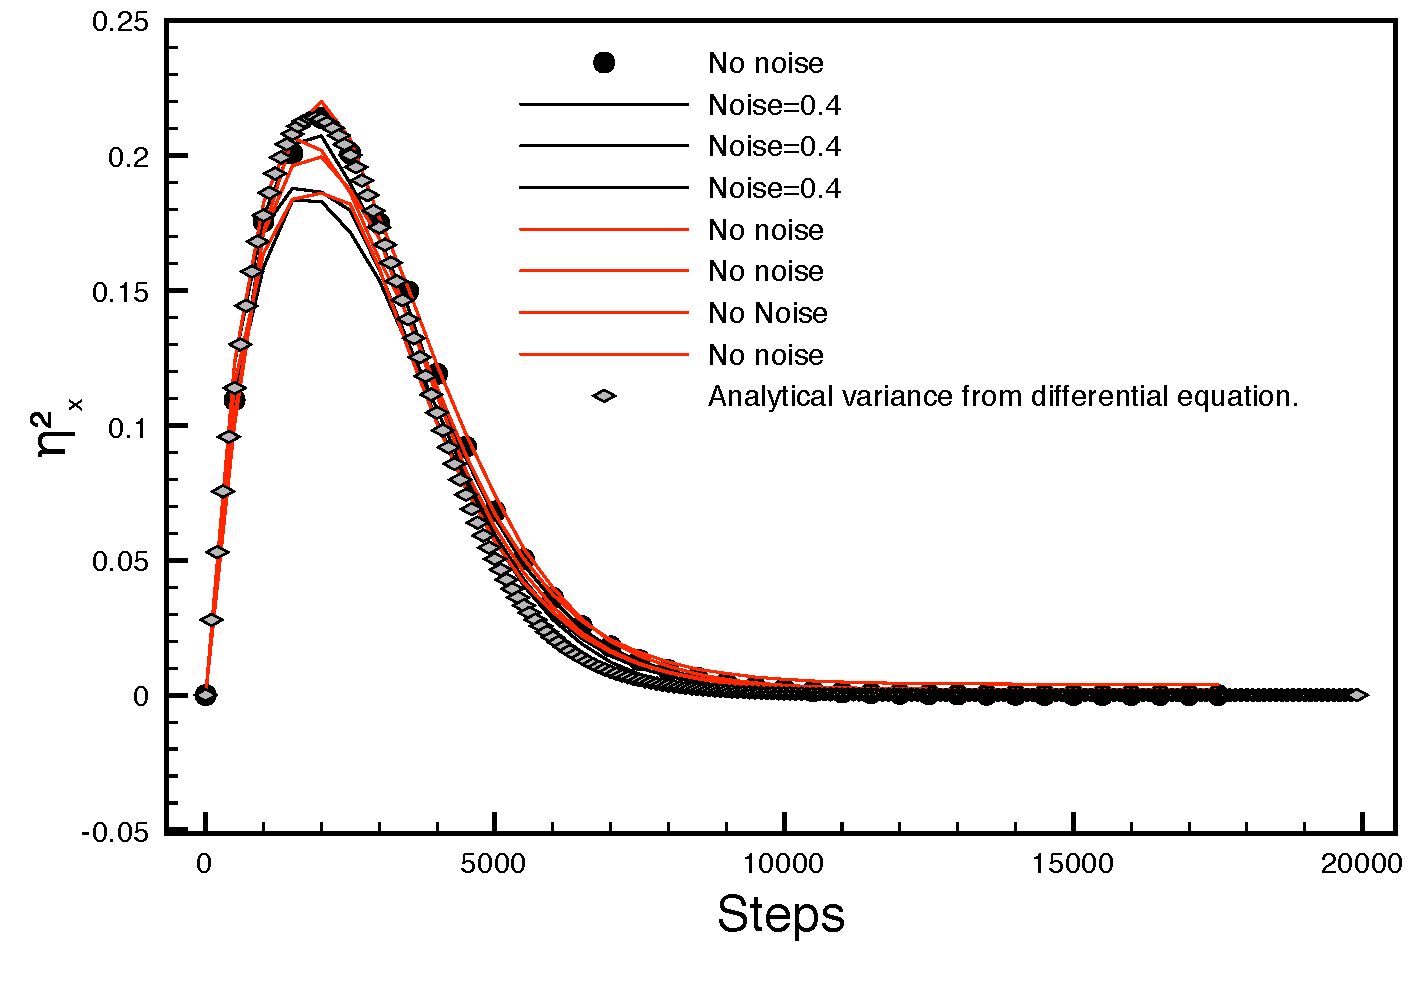
\includegraphics[width=9cm,height=8cm]{VarianceNoiseNonoiseAnalytical.pdf}
    \else
      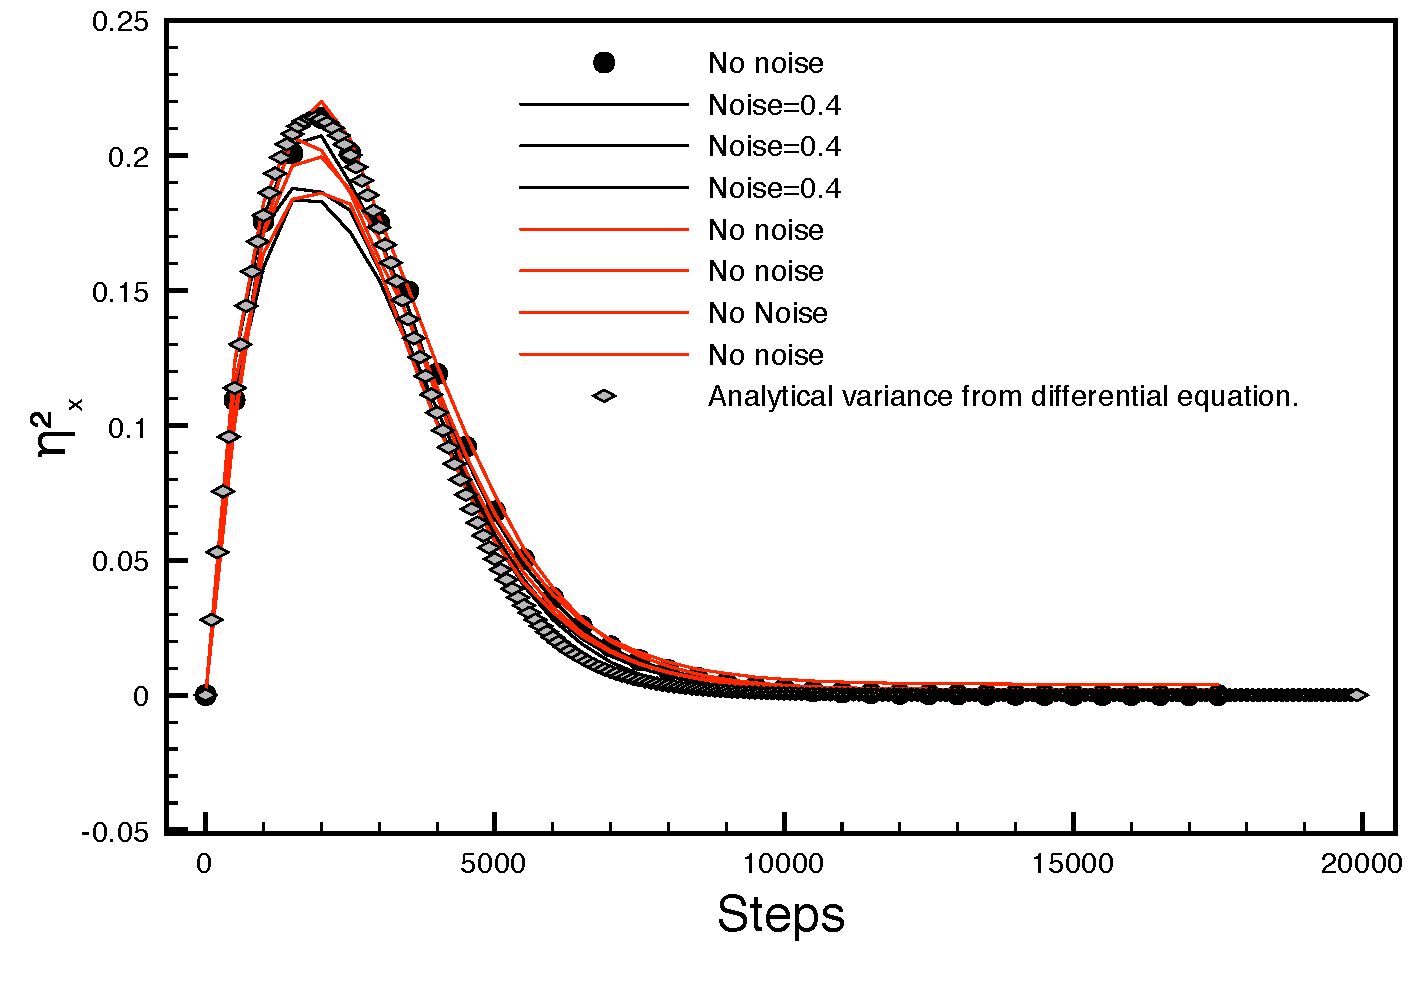
\includegraphics[width=9cm, height=8cm]{VarianceNoiseNonoiseAnalytical.pdf}
    \fi
    \caption{In this graph there are several plots for  noise $\eta_{x}^{2}=\sigma_{xx}/\langle x\rangle^2$. There are curves from the stochastic simulation and one, that is the solution of the analytical differential equation for variance. In the simulations for random drift $\bar{r}=2$, $s=1$ and the noise for $r$ is $0.4$(gaussian distribution), $n=1000$ and $i=10$. The simulation data were obtained with $1000$ simulations, which is not an enough large to have similar curves in each execution of the program.}
    \label{Fig7.5}
  \end{center}
  \end{figure}

\begin{figure}[H]
  \begin{center}
    \leavevmode
    \ifpdf
      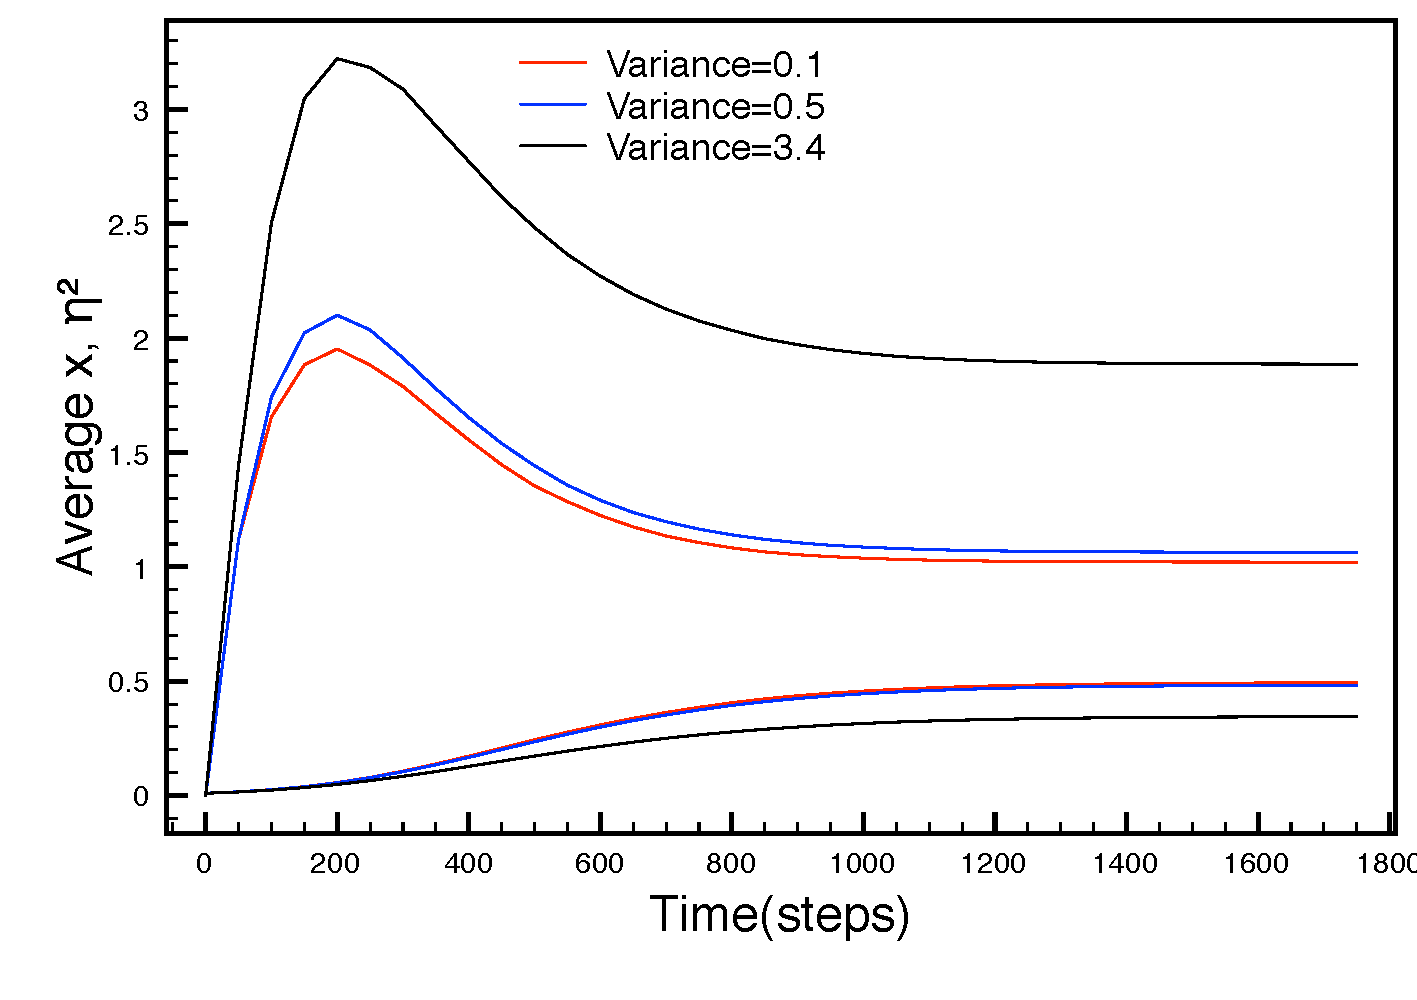
\includegraphics[width=9cm,height=8cm]{noisepopulation100.pdf}
    \else
      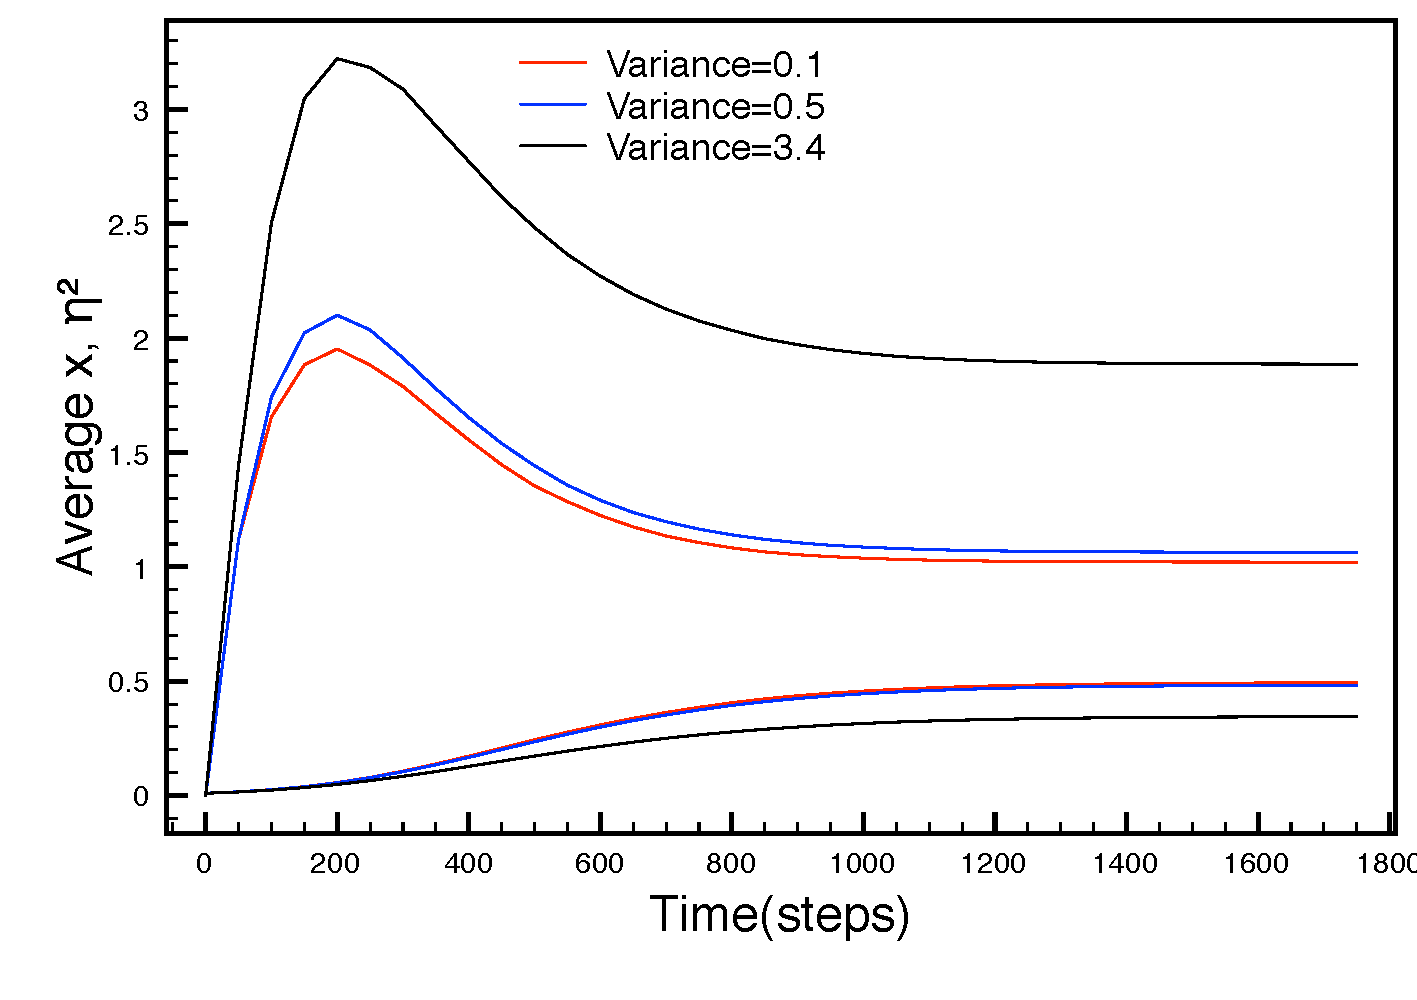
\includegraphics[width=9cm, height=8cm]{noisepopulation100.pdf}
    \fi
    \caption{In this graph there are several plots for  noise $\eta_{x}^{2}=\sigma_{xx}/\langle x\rangle^2$. In the simulations for random drift $\bar{r}=2$, $s=1$, and the random values for $r$ come from a gamma distribution with different variance for each curve. The population size is $n=100$ and the initial number of individual with fitness $r$ is  $i=1$. The simulation data were obtained with $10^4$ simulations.}
    \label{}
  \end{center}
  \end{figure}

\begin{figure}[H]
  \begin{center}
    \leavevmode
    \ifpdf
      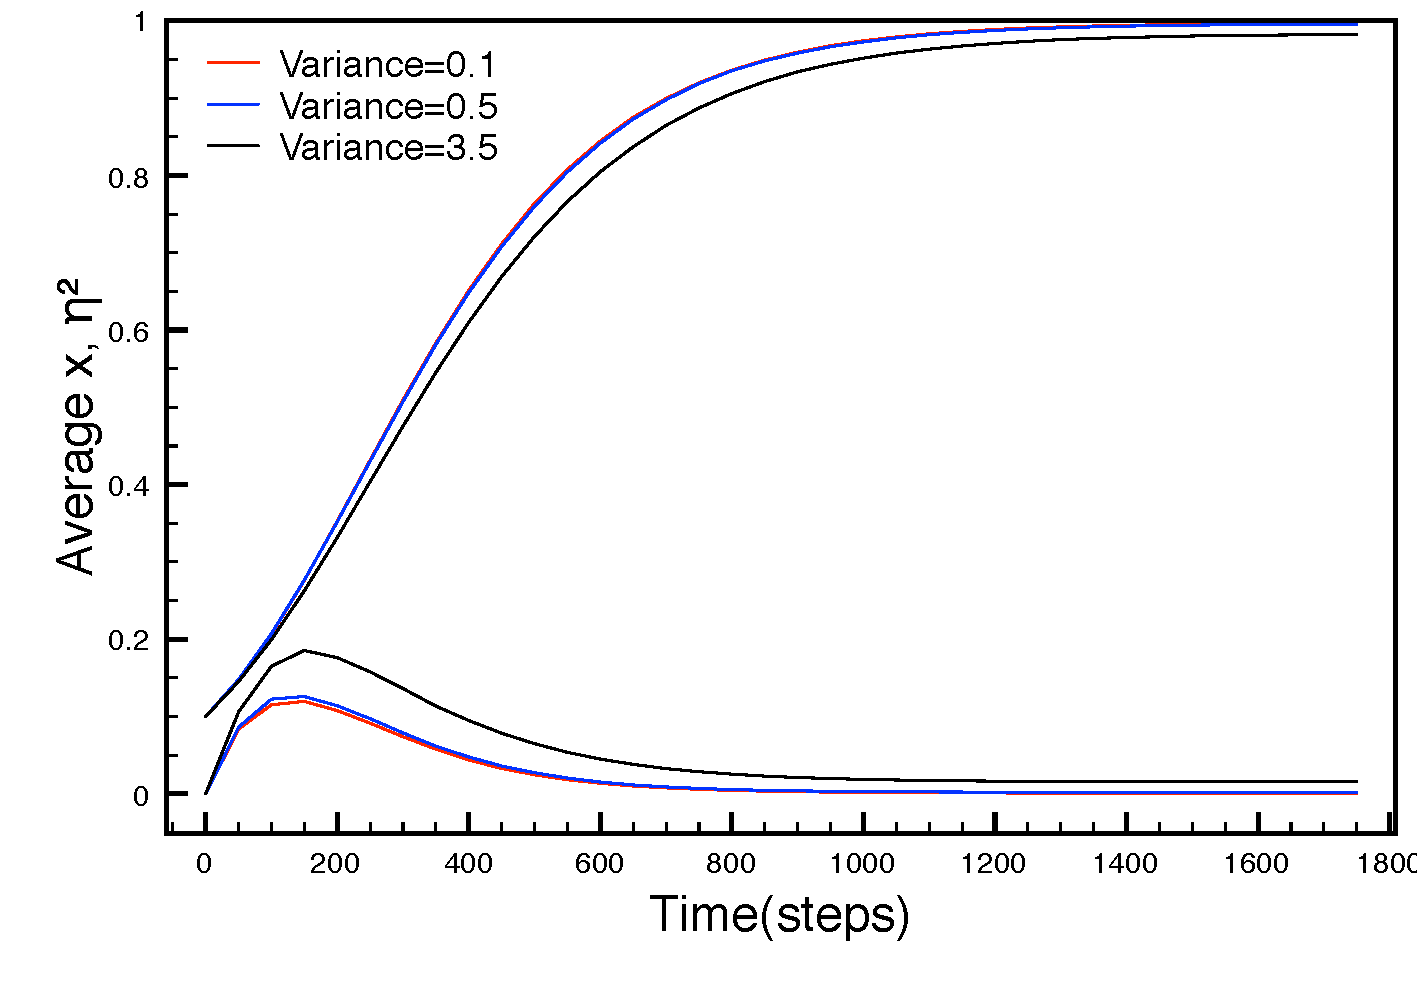
\includegraphics[width=9cm,height=8cm]{noise10010gammavariance.pdf}
    \else
      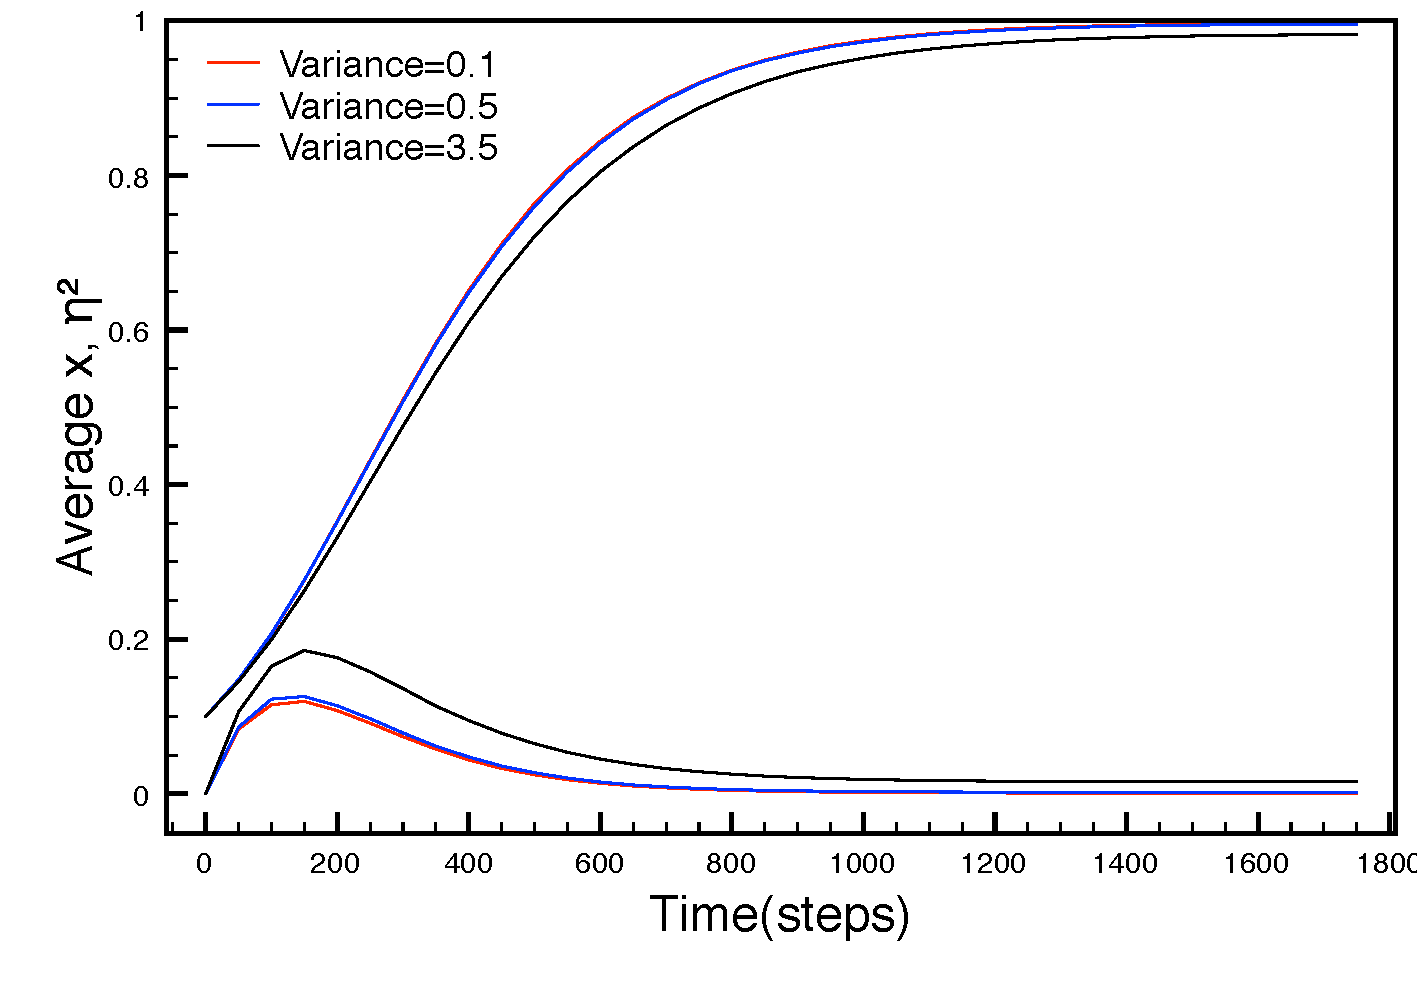
\includegraphics[width=9cm, height=8cm]{noise10010gammavariance.pdf}
    \fi
    \caption{In this graph there are several plots for  noise $\eta_{x}^{2}=\sigma_{xx}/\langle x\rangle^2$. In the simulations for random drift $\bar{r}=2$, $s=1$, and the random values for $r$ come from a gamma distribution with different variance for each curve. The population size is $n=100$ and the initial number of individual with fitness $r$ is  $i=10$. The simulation data were obtained with $10^4$ simulations.}
    \label{}
  \end{center}
  \end{figure}
  
\begin{figure}[H]
\begin{center}$
\begin{array}{cc}
a)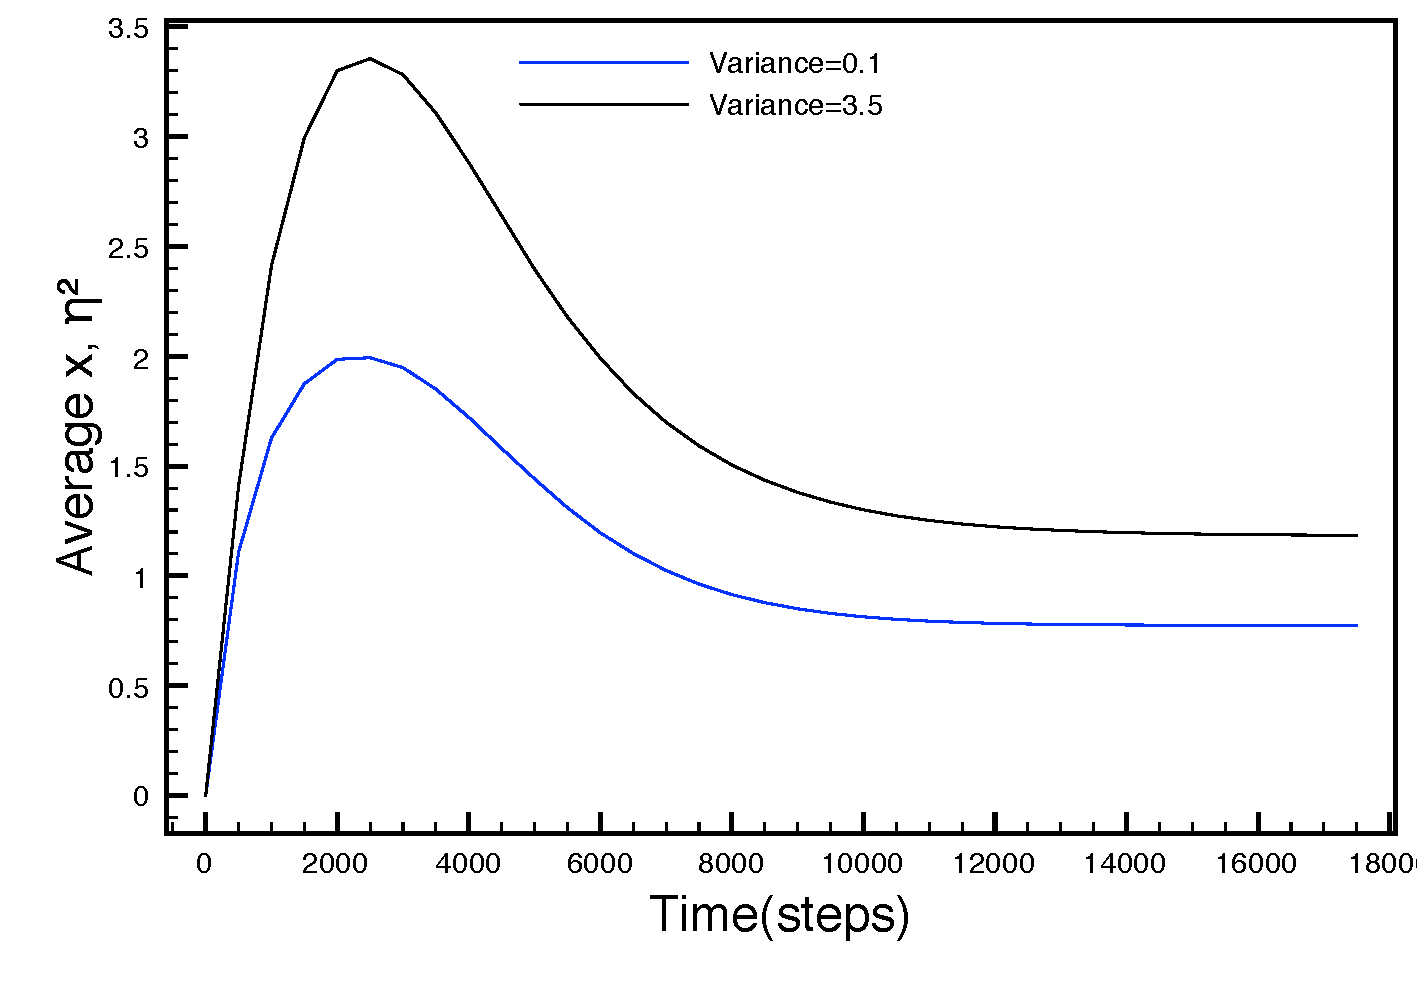
\includegraphics[width=2.5in]{VarianceTime10001noise.pdf} &
b)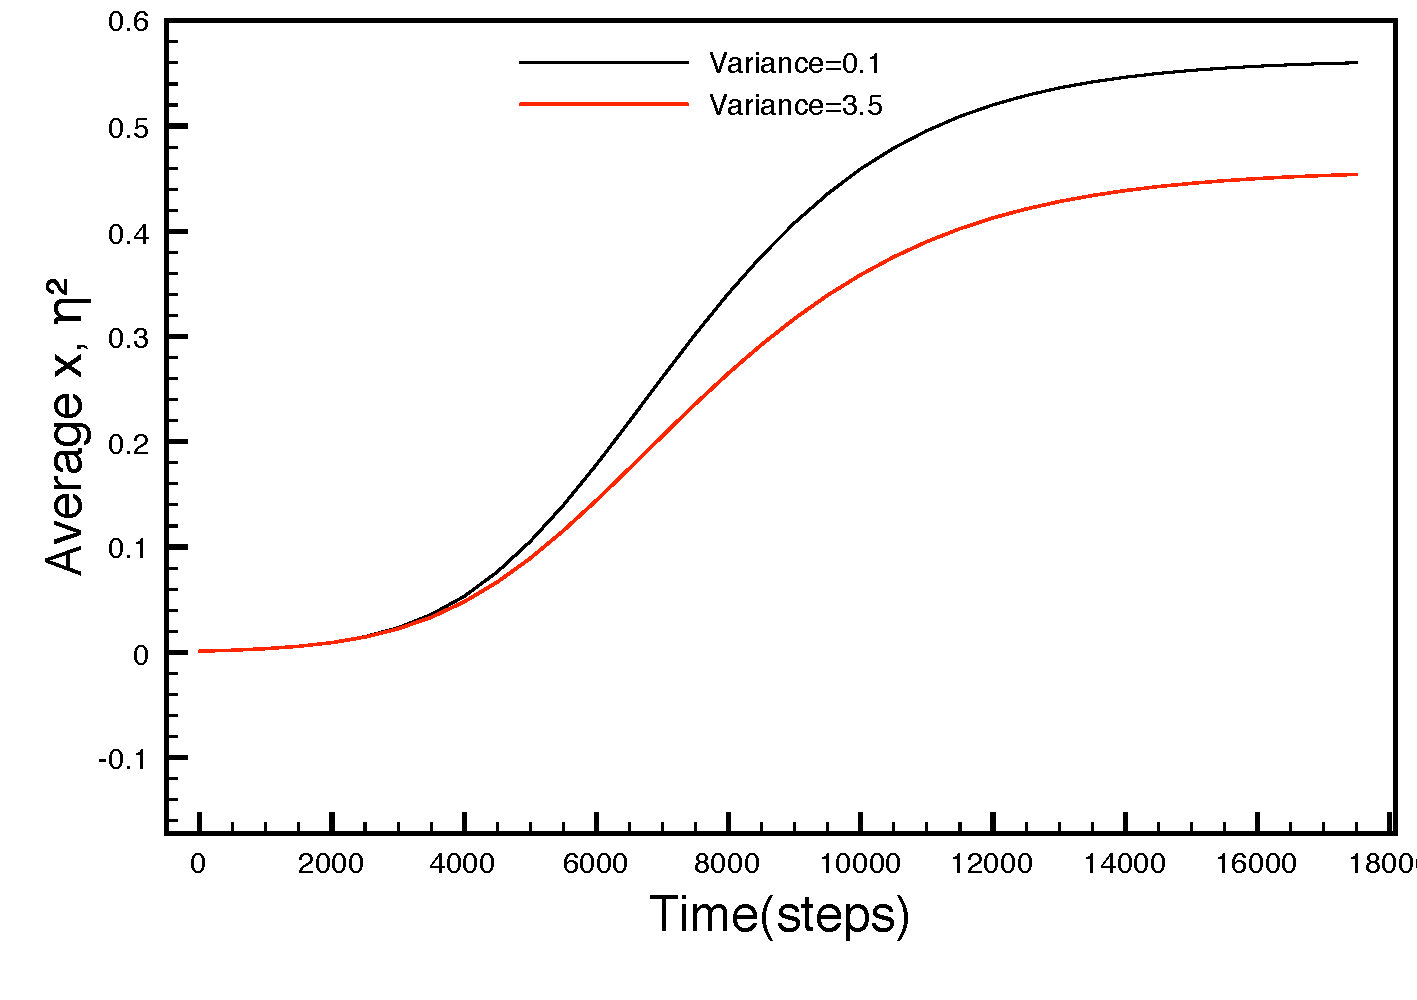
\includegraphics[width=2.7in]{AverageTime10001noise.pdf}
\end{array}$
\end{center}
\caption{In this graph there are several plots for  noise $\eta_{x}^{2}=\sigma_{xx}/\langle x\rangle^2$. In the simulations for random drift $\bar{r}=2$, $s=1$, and the random values for $r$ come from a gamma distribution with different variance for each curve. The population size is $n=1000$ and the initial number of individual with fitness $r$ is  $i=1$. The simulation data were obtained with $10^4$ simulations.a) Standard deviation curves. b) Average population fraction curves. It can be observed that the standard deviations and the difference in the population average are smaller than the case for $n=100$, which means that for large populations the effects of internal noise decrease.}
\label{}
\end{figure}



In this system of natural selection, fitness is not a deterministic variable, which affects the birth and death fluxes for $\bar{ x}$. Fitness depends on the protein expression  of each cell or individual.  The average equation for protein expression $\bar{p}$ 
\begin{equation}
	\frac{d \bar{p}}{dt}=\beta(\bar{y}_{1}, ...., \bar{y}_{k}) - \lambda \bar{p}.
\end{equation} 
Where $\beta(\bar{y}_{1}, ...., \bar{y}_{k})$ is a function of the $k$ reactions in the genetic network. We can consider the case where phenotypic proteins are not altered by the rest of metabolic network. 

For simplicity $s$ will be considered deterministic and $r(p)$ stochastic. 

Then, the matrices $\mathbf{A}$ and $\mathbf{B}$ for this system are

\begin{equation}
\begin{split}
\mathbf{A}&=\begin{pmatrix} -\lambda & 0 \\
\partial_{p}\frac{d\bar{x}}{dt} & \partial_{\bar{x}}\frac{d\bar{ x}}{dt}
\end{pmatrix}\;\; , \\ \mathbf{B}&=\begin{pmatrix}\beta(\bar{y}_{1}, ...., \bar{y}_{k}) + \lambda\bar{p} & 0 \\
0 & \frac{\bar{x}(1-\bar{x})}{n(r(\bar{p} )\bar{x}+ s(1-\bar{x}))}(r(\bar{p})+ s)
\end{pmatrix}
\end{split}
\end{equation}
Therefore the variance equations are
\begin{gather}
\frac{d\sigma_{pp}}{dt}=-2\lambda\sigma_{pp}+\beta(\bar{y}_{1}, ...., \bar{y}_{k})+ \lambda\bar{p} \;\; , \;\; \frac{d\sigma_{px}}{dt}=\sigma_{pp}\partial_{\bar{ p}}\frac{d\bar{ x}}{dt} + \sigma_{xp}\partial_{\bar{x}}\frac{d\bar{x}}{dt} - \lambda\sigma_{xp} \notag \\
\frac{d\sigma_{xx}}{dt}=2\left(\partial_{\bar{p}}\frac{d\bar{x }}{dt} \sigma_{xp} + \sigma_{xx}\partial_{\bar{x}}\frac{d\bar{ x}}{dt} \right) + \frac{\bar{x}(1-\bar{x})}{n(r(\bar{p})\bar{x}+ s(1-\bar{x}))}(r(\bar{p})+ s)
\end{gather}
We are interested in the direct relation of fitness variability with population dynamics. To examine this, we can considerate that for each generation of cells(a birth and death event), all of them would have reached its internal steady state, which is valid  because of the large difference between the times for protein events and a birth and death cell. Hence $\sigma_{pp}$ is a time constant respect to the Moran process.
\begin{equation}
0=-2\lambda\sigma_{pp}+\beta(\bar{y}_{1}, ...., \bar{y}_{k})+ \lambda\bar{p} 
\end{equation} 
 

%%% ----------------------------------------------------------------------

%%% Local Variables: 
%%% mode: latex
%%% TeX-master: "../thesis"
%%% End: 
